% ACL 2023 Template
\documentclass[11pt]{article}
\usepackage[review]{acl}
\usepackage{times}
\usepackage{latexsym}
\usepackage[T1]{fontenc}
\usepackage[utf8]{inputenc}
\usepackage{microtype}
\usepackage{graphicx}
\usepackage{booktabs}
\usepackage{enumitem}
\usepackage{amsmath}
\usepackage{amssymb}
\usepackage{placeins}
\usepackage{multirow}
\usepackage{float}
\usepackage{stfloats}
\usepackage{alphalph}
\usepackage{tcolorbox}
\tcbuselibrary{breakable}

\graphicspath{{../chart/}}

\title{Depth Profiling: Classifying Recursive Generation Depth\\in Base-Model LLM Text}

\author{Anonymous}

\begin{document}
\maketitle

% Abstract — Depth Profiling of Recursive LLM Generation Chains
\begin{abstract}
As large language model (LLM) outputs re-enter training corpora and seed further generation, understanding how recursive generation reshapes text distributions is critical for data provenance and corpus curation. Existing detectors answer only the binary human-or-machine question, ignoring \emph{generation depth}; we introduce \emph{depth profiling} to address this gap.
We decompose distributional drift under recursive generation into location and shape components. Across eight base-model generators from five families, negative log-likelihood (NLL) location features drift monotonically with depth while shape features remain near-stationary---an effect-size gap exceeding $8{\times}$ ($d{=}0.74$--$1.05$ vs.\ $d < 0.10$). We term this asymmetry the \emph{differential depth response} (DDR).
Prior work documents \emph{what converges}; the central finding here is \emph{what is approximately preserved}: shape stability complements location drift for ordinal depth grading without per-generator calibration. A lightweight ensemble achieves leak-free binary F1\,=\,0.694 under 8-generator leave-one-generator-out evaluation; cross-model chains reach F1\,=\,0.830.
Instruction tuning compresses DDR and bounds current applicability to base models\footnote{Code and data are available at \url{https://anonymous.4open.science/r/gen-depth-fingerprint-3FB3/}.}.
\end{abstract}


\section{Introduction}
\label{sec:introduction}

\looseness=-1 An estimated 7--17\% of recent scientific publications already contain substantial LLM-modified content \cite{mapping_llm_science,monitoring_ai_review}. As these outputs re-enter training corpora \cite{dolma,fineweb} and seed further generation, text accumulates at varying \emph{generation depths}; each successive cycle reshapes distributional properties in ways that matter for data provenance, corpus auditing, and contamination monitoring in base-model pretraining corpora \cite{ccnet,dsir} as well as model collapse analysis \cite{curse_of_recursion,strong_model_collapse}. Understanding \emph{how} recursive generation alters text distributions, and which properties change versus which are preserved, is therefore a prerequisite for principled corpus curation, yet current methods address only binary human-or-machine detection \cite{detectgpt,fast_detectgpt,binoculars,ld_score}.
Base models provide the cleanest substrate to isolate depth effects from alignment-induced changes.
We find that recursive generation produces a decomposable depth profile: distributional \emph{location} drifts with depth while \emph{shape} remains stable across generators, an asymmetry sufficient for cross-generator depth prediction.

\looseness=-1 Distributional compression under recursive generation is well-documented \cite{curious_decline,broken_telephone,markovian_chains}, yet existing analyses characterize \emph{that} and \emph{why} convergence occurs without decomposing what drifts from what is preserved.
We introduce \emph{depth profiling} (coarse ordinal classification into gen-0\,/\,gen-1\,/\,gen-2+) and decompose this compression into structurally distinct components.
Across eight base-model generators spanning five architectural families (0.6B--8B), the NLL distribution's central tendency---mean entropy (per-token NLL under a fixed reference model, not information-theoretic entropy; \S\ref{sec:features}) and lexical diversity---drifts monotonically with depth, while its shape (entropy extremes, tail structure) remains ${\geq}8{\times}$ more stable ($d{=}0.74$--$1.05$ vs.\ $d < 0.10$; entropy std is intermediate at $d{=}0.46$).
We term this location/shape asymmetry the \emph{differential depth response} (DDR; Figure~\ref{fig:ddr-trajectory}), an empirical regularity of base-model autoregressive generation that is mechanistically distinct from model collapse \cite{curse_of_recursion}. Model collapse erodes tail coverage via weight updates; DDR instead analyzes fixed-parameter inference chains.
The stationary shape component complements location drift for depth prediction without per-generator calibration.

\begin{figure*}[t!]
\centering
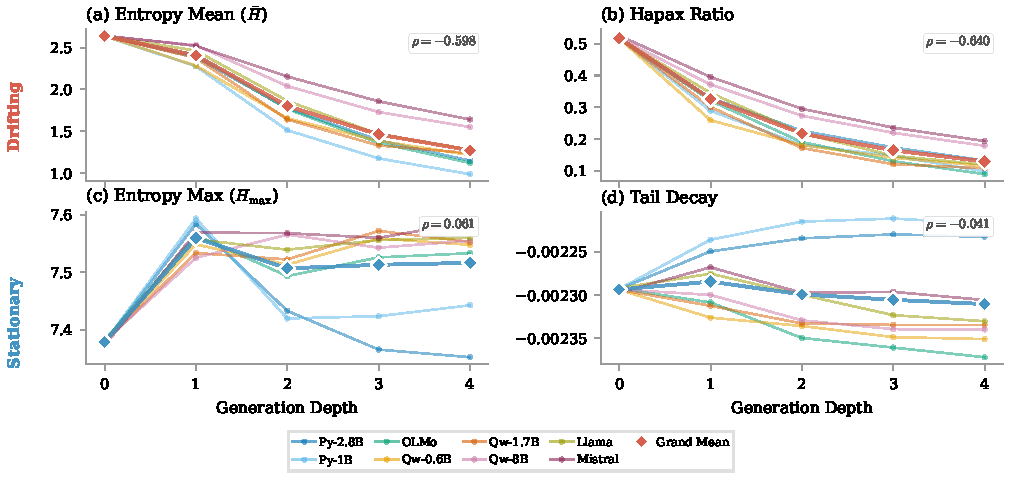
\includegraphics[width=\textwidth]{fig_ddr_trajectory.pdf}
\caption{Feature trajectories across generation depth ($y$-axis: $z$-scored feature values). \textbf{Top row (drifting)}: entropy mean and hapax ratio decline monotonically across all eight generators ($|\rho| > 0.59$). \textbf{Bottom row (stationary)}: entropy max and tail decay remain flat ($|\rho| < 0.07$). Colored lines: individual generators; diamonds: cross-generator mean (red for drifting, blue for stationary). This dichotomy defines the DDR.}
\label{fig:ddr-trajectory}
\end{figure*}
We focus on base (pretrained) models; instruction tuning degrades depth signal (Appendix~\ref{app:instruct}).
Figure~\ref{fig:framework} summarizes the pipeline: recursive generation chains (\S\ref{sec:generation}), feature extraction with DDR partitioning (\S\ref{sec:features}), and leave-one-generator-out (LOGO) evaluation (\S\ref{sec:evaluation}).

\looseness=-1 As a proof of concept, a lightweight 7-feature ensemble informed by DDR achieves leak-free binary F1\,=\,0.694 (macro-averaged LOGO; pooled: 0.705), matching multi-detector ensembles (0.708) at ${\sim}2.4\times$ lower cost; an end-to-end QLoRA \cite{qlora} (Quantized Low-Rank Adaptation) classifier reaches 3-class F1\,=\,0.905 (within-model 5-fold CV; Appendix~\ref{app:qlora}), and the depth signal thus extends well beyond handcrafted features.

Our contributions:
\begin{enumerate}[nosep,leftmargin=*]
    \item \textbf{Empirical decomposition (DDR).} Across eight generators from five families, we decompose inference-chain drift into two primary response zones (drifting, $d{=}0.74$--$1.05$; near-stationary, $d < 0.10$) plus one intermediate feature ($d{=}0.46$). Where prior work documents \emph{what converges} \cite{curious_decline,markovian_chains}, DDR identifies \emph{what is approximately preserved}, an empirical regularity with analytical utility for depth classification without per-generator calibration.
    \item \textbf{Task formulation and evaluation suite.} We define generation depth classification as an ordinal prediction task and construct a controlled dataset of 37K texts from eight generators across five families (0.6B--8B; exploratory evidence extends to 14B, Appendix~\ref{app:9gen-scale}), with leave-one-generator-out cross-validation as the primary evaluation protocol.
    \item \textbf{Scope characterization.} Systematic evaluation across temperature, prompt type, instruction tuning, model scale, domain transfer, and perturbation robustness maps the operational envelope of depth profiling.
\end{enumerate}

\begin{figure*}[t]
\centering
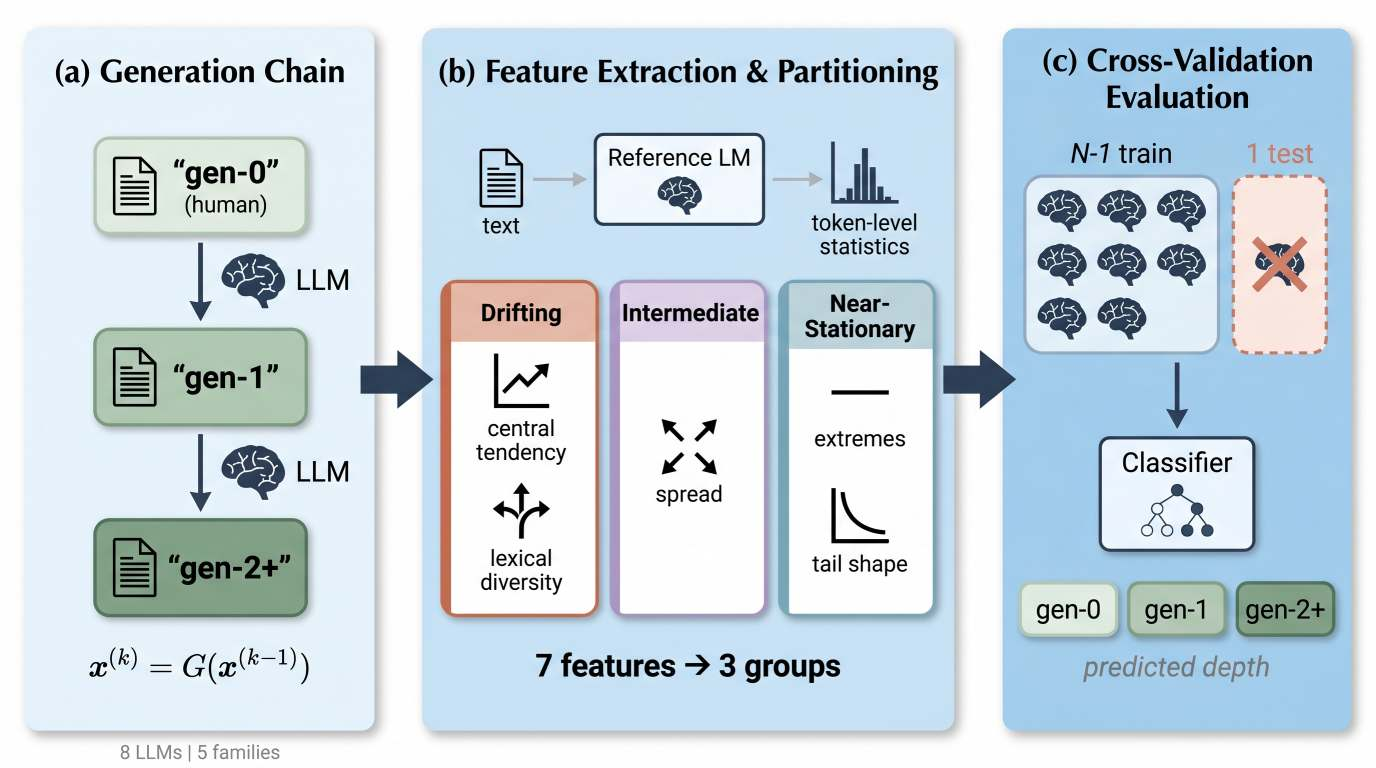
\includegraphics[width=\textwidth]{fig2_framework.pdf}
\caption{Depth profiling pipeline. (a)~Human seeds are iteratively fed through generator $G$ to produce chains of increasing depth. (b)~Seven features extracted from NLL distributions group into three DDR zones: drifting (red), intermediate (purple), near-stationary (blue). (c)~LOGO evaluation holds out one generator for testing.}
\label{fig:framework}
\end{figure*}

\section{Related Work}
\label{sec:related}

\paragraph{AI-generated text detection.}
\looseness=-1 Detection methods span zero-shot scoring \cite{detectgpt,fast_detectgpt,binoculars,dna_gpt}, learned classifiers \cite{ghostbuster,ld_score,reliable_detection}, and surprisal-based approaches \cite{diveye,xu_spectrum_detection}; see \citet{wu_survey_2025} for a survey.
Recent work moves beyond binary detection---multi-generator attribution \cite{semeval2024_task8}, collaboration roles \cite{beyond_binary}, joint detection-attribution \cite{two_birds}---but all taxonomize by \emph{source} or \emph{production mode}, not recursive generation \emph{depth}.
Recent work reframes detection as an out-of-distribution problem \cite{human_texts_outliers}; depth profiling differs in targeting ordinal depth rather than binary membership, with cross-generator transfer as the evaluation axis.
We introduce ordinal depth classification \cite{gutierrez_ordinal_survey,coral_ordinal} as a complementary task; repurposing existing detection scores as depth predictors reveals high cross-generator variance (binary F1\,=\,0.54--0.71; Table~\ref{tab:baselines}).

\paragraph{Model collapse and iterative generation.}
\looseness=-1 Self-consuming generative models lose distributional coverage via training-loop parameter updates \cite{self_consuming_mad,curse_of_recursion,strong_model_collapse,dohmatob_tale_of_tails,schaeffer_collapse_position}; we instead examine \emph{inference chains} where parameters are fixed.
Concurrent iterative-generation studies document complementary phenomena: paraphrasing chains show factuality degradation \cite{broken_telephone}, Markovian analysis bounds distinguishable depth to ${\sim}$3 classes \cite{markovian_chains}, and attractor cycle evidence emerges \cite{attractor_cycles}.
DDR differs in chain type (non-paraphrastic continuation), analysis lens (location/shape decomposition identifying what is \emph{preserved}), and downstream utility (shape stability enables cross-generator classification without calibration); a detailed comparison appears in Appendix~\ref{app:iterative-comparison}.

\paragraph{Diversity, stylometry, and provenance.}
\looseness=-1 Declining lexical diversity under recursive generation \cite{curious_decline,writing_diversity} aligns with the monotonic TTR and hapax ratio decline we observe; these classical stylometric features \cite{stamatatos_survey} constitute DDR's drifting component.
Data curation relies on quality signals \cite{dsir,ccnet}; generation depth offers a complementary provenance axis.
Watermarking \cite{watermark_llm,synthid_text} requires generator cooperation and degrades across multi-step chains \cite{chainwash}; our post-hoc approach requires no generation-time modification.
Our NLL tail analysis extends probability-based membership inference \cite{min_k_percent,koike_mia_detection} from binary membership to ordinal depth.

\section{Method}
\label{sec:method}

\begin{table}[t!]
\centering
\footnotesize
\caption{Seven distributional features. ``Entropy'' features are per-token NLL under Pythia-410M (\S\ref{sec:features}); surface features require no reference model. DDR analysis (\S\ref{sec:results-differential}) reveals entropy mean, TTR, and hapax ratio drift with depth while entropy max, min, and tail decay remain near-stationary; entropy std is intermediate.}
\label{tab:features}
\setlength{\tabcolsep}{4pt}
\begin{tabular}{@{}llp{3.0cm}@{}}
\toprule
\textbf{Feature} & \textbf{Source} & \textbf{Measures} \\
\midrule
\texttt{entropy\_mean} \textit{\scriptsize(NLL)} & Ref.\ NLL & Central tendency of token surprise \\
\texttt{entropy\_std} \textit{\scriptsize(NLL)}  & Ref.\ NLL & Spread of token surprise \\
\texttt{entropy\_max} \textit{\scriptsize(NLL)}  & Ref.\ NLL & Maximum token surprise \\
\texttt{entropy\_min} \textit{\scriptsize(NLL)}  & Ref.\ NLL & Minimum token surprise \\
\texttt{tail\_decay}   & Ref.\ NLL & Log-prob decay slope (ranks 100--1K) \\
\midrule
\texttt{ttr}           & Surface & Type-token ratio \\
\texttt{hapax\_ratio}  & Surface & Proportion of hapax legomena \\
\bottomrule
\end{tabular}
\end{table}

\subsection{Task Formulation}
\label{sec:task}

Given a text $x$, we predict its \emph{generation depth} $d \in \{0, 1, 2{+}\}$: human-written ($d{=}0$), first-generation LLM output ($d{=}1$), or text produced by two or more recursive LLM generations ($d{=}2{+}$).
A generation chain of depth $k$ is defined recursively: $x^{(0)} \sim \mathcal{C}_0$ (human corpus), $x^{(k)} = G(x^{(k-1)})$ for $k \geq 1$, where $G$ denotes stochastic autoregressive generation.
Depths beyond 2 are merged into $2{+}$ because feature convergence compresses inter-class margins at deeper levels (\S\ref{sec:results-differential}).

\subsection{Generation Chain Construction}
\label{sec:generation}

\looseness=-1 We construct generation chains using eight generators spanning five model families: \textbf{Pythia} (2.8B, 1B) \cite{pythia}, \textbf{OLMo} (OLMo-2-1B) \cite{olmo}, \textbf{Qwen} (Qwen3-1.7B, Qwen3-0.6B, Qwen3-8B-Base) \cite{qwen3}, \textbf{Llama} (Llama-3.2-3B) \cite{llama3}, and \textbf{Mistral} (Mistral-7B-v0.3) \cite{mistral7b}.
\looseness=-1 These span a 13$\times$ parameter range (0.6B--8B) across five architectures; Qwen's overrepresentation (3/8) is a limitation mitigated by leave-one-family-out (LOFO) evaluation (F1\,=\,0.686; \S\ref{sec:results-classification}).

\looseness=-1 For each generator, we sample approximately 1{,}000 seed passages from English Wikipedia as $\mathcal{C}_0$.
The same seed pool serves as gen-0 for all generators, controlling for input content; in LOGO evaluation this creates a potential train--test overlap for gen-0, addressed by our binary evaluation excluding gen-0 entirely (\S\ref{sec:results-baselines}).
Each seed is iteratively fed through the generator to produce a chain of depth 4 (i.e., gen-0 through gen-4), using the prompt ``\texttt{Continue the following text: \{text\}}''.
We generate up to depth~4 to empirically confirm convergence: 5-class LOGO yields macro F1\,$\approx$\,0.50, with depths 2--4 near-indistinguishable (gen-2/gen-3 per-class F1\,$<$\,0.27; Appendix~\ref{app:finer-depth}). This motivates the gen-2+ class collapse.
All generation uses temperature $\tau{=}0.7$, nucleus sampling with $p{=}0.9$, and maximum length of 256 new tokens.
After filtering chain breaks and passages too short for feature extraction, 37{,}058 texts remain across all depths (Appendix~\ref{app:dataset-stats}); depths 2--4 are collapsed into $2{+}$.

\subsection{Feature Extraction}
\label{sec:features}

\paragraph{Terminology.} Throughout this paper, we refer to per-token cross-entropy loss under a fixed reference model as ``entropy'' for conciseness; these are reference-model NLL values, not true information-theoretic entropy of the generating distribution.

We use interpretable distributional statistics so that the DDR partition remains transparent; end-to-end neural features improve classification ($+$10.0\,pp; Appendix~\ref{app:qlora}) but obscure the decomposition (LOFO confirms both feature groups contribute independently; Appendix~\ref{app:lofo}).

\looseness=-1 We extract seven distributional features per text (Table~\ref{tab:features}), covering the NLL distribution's location, spread, extremes, and tail structure, plus two reference-free surface diversity measures; six additional NLL statistics were rejected for redundancy ($|r| > 0.65$, $\Delta$F1\,$\leq$\,$-0.011$; Appendix~\ref{app:feature-candidate}).

\paragraph{Reference-model features.}
\looseness=-1 A held-out reference model (Pythia-410M, chosen to be smaller than all generators) computes per-token negative log-likelihood (NLL) for each text.
Cross-family reference validation (Appendix~\ref{app:cross-ref}) shows F1 spread of only 0.013 across Pythia, OLMo, and Qwen references, so DDR is reference-model agnostic; however, all tested references are causal LMs.
From the resulting NLL sequence, we extract five statistics: mean, standard deviation, maximum, and minimum of the token-level NLL, plus tail\_decay (the slope of the vocabulary-level averaged log-probability distribution in ranks 100--1000), which captures the power-law regime where depth-induced compression is most detectable.

\paragraph{Surface features.}
Two features capture lexical diversity without requiring a reference model: type-token ratio (TTR) and the proportion of words appearing exactly once (hapax\_ratio).

\paragraph{Feature complementarity.}
These features exhibit a \emph{differential depth response} (DDR), separating into drifting and non-drifting groups (\S\ref{sec:results-differential}; pairwise correlations in Appendix~\ref{sec:appendix-feature-correlation}).
TTR and hapax ratio are strongly correlated ($r = 0.97$); both are retained for marginal LOFO gains.

\subsection{Evaluation Protocol}
\label{sec:evaluation}

\paragraph{Cross-validation.}
\looseness=-1 We evaluate generalization via \textbf{LOGO} cross-validation: each fold holds out one generator entirely, so the classifier must generalize to a generator absent from training. This constitutes the strictest per-model protocol for assessing deployment against previously unseen generators.
LOGO does not isolate family-level effects; \textbf{LOFO} addresses this by holding out entire model families (binary F1\,=\,0.686; \S\ref{sec:results-classification}).
Generator subsets vary across experiments (Appendix~\ref{app:gen-subsets-section}).

\paragraph{Classifier.}
\looseness=-1 We use XGBoost \cite{xgboost} throughout ($n\_\text{estimators}{=}200$, $\max\_\text{depth}{=}6$, learning rate $0.1$; fixed without tuning), with identical hyperparameters across all methods in Table~\ref{tab:baselines}.
Alternative classifiers (CORAL \cite{coral_ordinal}, CORN \cite{corn_ordinal}, Frank-Hall \cite{frank_hall_ordinal}) yield comparable performance (Appendix~\ref{app:classifier}); hyperparameter sensitivity (max\_depth sweep) shows F1 variation $\leq$2.0\,pp, so discriminative power resides in the features, not the classifier.

\paragraph{Metrics and statistical testing.}
The primary metric is \textbf{macro-averaged F1} over the three depth classes, with 95\% bootstrap confidence intervals (CIs; $n{=}1{,}000$).
All $p$-values are two-sided with Bonferroni correction within each family of simultaneous tests.

\paragraph{Baselines.}
We compare the 7-feature ensemble against four single-score detection methods repurposed as depth predictors: Avg-LogProb, FastDetectGPT \cite{fast_detectgpt}, Binoculars \cite{binoculars}, and LD-Score \cite{ld_score}.
Each baseline score is used as a univariate feature in the same XGBoost framework under LOGO cross-validation to ensure a controlled comparison.

\paragraph{Length confound control.}
Since TTR and hapax\_ratio are mechanically length-dependent, we verify depth signal is not a length artifact via length-matched subsampling that equalizes length distributions across depth classes (\S\ref{sec:results-classification}; Appendix~\ref{app:length}).

\section{Results}
\label{sec:results}

\begin{figure}[t]
\centering
\includegraphics[width=\columnwidth]{fig_transfer_heatmap.pdf}
\caption{Cross-generator $8{\times}8$ transfer matrix (binary F1, gen-1 vs.\ gen-2+). Mean cross-generator F1\,=\,0.810 [95\% CI: 0.796, 0.822]; uniformly high off-diagonal values confirm depth signal transfers across five families without calibration.}
\label{fig:transfer-heatmap}
\end{figure}

\subsection{Depth Classification Performance}
\label{sec:results-classification}

\looseness=-1 The 7-feature ensemble achieves 3-class LOGO F1\,=\,0.762 (95\% CI [0.758, 0.766]; $N$\,=\,37{,}058) across eight generators from five families (Table~\ref{tab:logo-results}); cross-generator F1 spread of 9.1\,pp captures generator selection uncertainty.
This 3-class metric is inflated by shared gen-0 seeds (per-class gen-0 F1\,$\approx$\,0.94; \S\ref{sec:generation}); we therefore report \textbf{leak-free binary F1} (gen-1 vs.\ gen-2+)\,=\,0.694 (CI [0.688, 0.700]) throughout, excluding gen-0 entirely.
Per-generator binary F1 ranges from 0.633 (Mistral-7B) to 0.724 (Pythia-2.8B; std.\ dev.\ 0.028), with the primary difficulty at the gen-1\,/\,gen-2+ boundary (Appendix~\ref{app:confusion}).

\paragraph{Cross-model generalization.}
\looseness=-1 Cross-model chains (randomly selected generator per step) yield binary F1\,=\,0.830 (95\% CI [.818, .841]; Appendix~\ref{app:cross-model-detail}) under 5-generator LOGO.\footnote{Pythia-2.8B/1B, OLMo-2-1B, Qwen3-0.6B/1.7B; generator-level LOGO with bootstrap CIs ($n$\,=\,1{,}000).}
Single-generator transfer confirms the signal is not a mixed-chain artifact (mean transfer F1\,=\,0.810; Figure~\ref{fig:transfer-heatmap}; full $8{\times}8$ matrix: Appendix~\ref{app:transfer}; LOFO\,=\,0.686).
ANOVA confirms generator identity contributes ${<}1$\% of feature variance ($\eta^2_{\text{gen}} \leq 0.009$; Appendix~\ref{app:cross-model-detail}).
A scale effect emerges: smaller models achieve higher F1 (Pythia-2.8B: 0.724 vs.\ Mistral-7B: 0.633), partly due to same-family affinity with the Pythia-410M reference (spread $\leq$0.013; \S\ref{sec:results-differential}).
An end-to-end QLoRA classifier reaches 3-class F1\,=\,0.905 (within-model 5-fold CV; $+$10.0\,pp; Appendix~\ref{app:qlora}), evidence that additional depth signal resides in token-level representations. On instruct data, QLoRA recovers to 0.89--0.91 (within-model; Appendix~\ref{app:instruct}).

\paragraph{Confound controls.}
\looseness=-1 Length-matched subsampling yields binary F1\,=\,0.724 (vs.\ 0.770; Appendix~\ref{app:length}); independent-seed evaluation with disjoint pools (F1\,=\,0.680; Appendix~\ref{app:seed-control}), so the classifier captures generative degradation rather than seed-specific content.

\paragraph{Error analysis.}
\looseness=-1 The gen-1\,/\,gen-2+ boundary is the primary failure point: depth-2 samples (the shallowest within the 2+ class) exhibit the highest error rate (48.4\%), decreasing monotonically to 20.3\% at depth-4 (Appendix~\ref{app:error-analysis}) due to insufficient accumulated drift beyond the large gen-0$\to$gen-1 distributional shift.
Error rates decrease monotonically at deeper generations ($\leq$29.2\% at gen-3+); DDR signal thus strengthens with chain length.

\begin{table}[t]
\centering
\footnotesize
\caption{8-generator LOGO macro-F1 (bootstrap 95\% CIs, $n$\,=\,1{,}000). Binary F1 excludes gen-0. $^{\dagger}$3-class F1 has upward bias from shared gen-0 seeds; independent-seed controls confirm the signal (F1\,=\,0.680; Appendix~\ref{app:seed-control}).}
\label{tab:logo-results}
\resizebox{\columnwidth}{!}{%
\begin{tabular}{@{}llcccc@{}}
\toprule
\textbf{Model} & \textbf{Family} & \textbf{Params} & \textbf{Bin F1} & \textbf{95\% CI} & \textbf{3-class F1}$^{\dagger}$ \\
\midrule
Pythia-2.8B     & Pythia  & 2.8B & \textbf{0.724} & [.707, .742] & 0.798 \\
Pythia-1B       & Pythia  & 1.0B & 0.718 & [.700, .735] & \textbf{0.806} \\
Qwen3-1.7B     & Qwen    & 1.7B & 0.709 & [.693, .726] & 0.772 \\
Llama-3.2-3B   & Llama   & 3.2B & 0.697 & [.680, .713] & 0.775 \\
OLMo-2-1B      & OLMo    & 1.5B & 0.695 & [.679, .711] & 0.781 \\
Qwen3-8B       & Qwen    & 8.2B & 0.692 & [.674, .708] & 0.714 \\
Qwen3-0.6B     & Qwen    & 0.6B & 0.691 & [.673, .709] & 0.780 \\
Mistral-7B     & Mistral & 7.0B & 0.633 & [.617, .648] & 0.682 \\
\midrule
\multicolumn{3}{l}{\textbf{Average (8-gen LOGO)}} & \textbf{0.694} & [.688, .700] & \textbf{0.762} \\
\multicolumn{3}{l}{\textbf{LOFO (family-level)}} & 0.686 & --- & --- \\
\bottomrule
\end{tabular}}
\end{table}

\subsection{Differential Depth Response}
\label{sec:results-differential}

\paragraph{Formal definition.}
\looseness=-1 For feature $f$ measured across depths $d \in \{0,1,2{+}\}$, we define its \emph{depth sensitivity} as $\text{DDR}(f) = |\rho(\text{depth}, f)|$, where $\rho$ is Spearman correlation over all per-text measurements.
A feature is classified as \emph{drifting} if Cohen's $d > 0.50$ between adjacent depths, or \emph{stationary} if $d < 0.15$; the two-cluster structure is robust across $\varepsilon \in [0.10, 0.75]$ ($k$-means silhouette\,=\,0.660, $p{=}0.030$; exhaustive split enumeration ranks this partition first; independent replication in all eight generators; Appendix~\ref{app:ddr-validation}).
\looseness=-1 Recursive inputs grow increasingly self-typical~\citep{markovian_chains}; this predicts location drift with shape invariance (confirmed across nucleus, greedy, and top-$k$ strategies; Appendix~\ref{app:decoding-strategy}).

\looseness=-1 Figure~\ref{fig:ddr-trajectory} reveals the dichotomy: central-tendency features (entropy mean, TTR, hapax ratio) decline monotonically with depth, while shape features (entropy max, tail decay, entropy min) remain flat (per-feature distributions: Appendix~\ref{app:feature-distributions}; qualitative chain example: Appendix~\ref{app:qualitative}).
The partition is binary ($k{=}2$; silhouette\,=\,0.660), with entropy std as the sole \emph{intermediate} member ($d{=}0.46$, $|\rho|{=}0.16$), distinct from three near-stationary features ($d < 0.10$; Appendix~\ref{app:ddr-validation}).

\begin{figure}[t]
\centering
\includegraphics[width=\columnwidth]{fig1_differential_response.pdf}
\caption{Differential depth response (DDR). Drifting features (red; $|\rho| > 0.60$, effect size $d{=}0.74$--$1.05$) shift monotonically with generation depth; near-stationary features (blue; $d \leq 0.10$) are approximately preserved; entropy std (purple; $d{=}0.46$) is intermediate. Diamonds: cross-generator means; dots: per-generator values.}
\label{fig:feature-drift}
\end{figure}

\looseness=-1 Pooled Spearman correlations corroborate the split: drifting features show $|\rho| > 0.60$ (hapax ratio $-0.64$, TTR $-0.62$, entropy mean $-0.60$) vs.\ $|\rho| \leq 0.16$ for entropy max and tail decay; entropy min reaches $|\rho|{=}0.40$ due to its gen-0/gen-1 boundary sensitivity (discussed below). This persistent magnitude gap defines the DDR partition (Figure~\ref{fig:feature-drift}).

\begin{figure}[t]
\centering
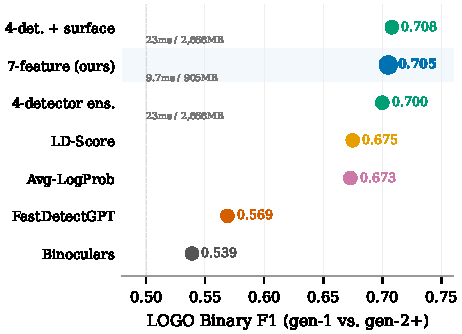
\includegraphics[width=\columnwidth]{fig3_baseline_comparison.pdf}
\caption{LOGO binary F1 vs.\ inference cost (8-gen pooled). The 7-feature ensemble (one 410M model) matches multi-detector ensembles (1.4B total) at ${\sim}2.4\times$ lower cost. RTX 5090 timings.}
\label{fig:baseline-ci}
\end{figure}

\paragraph{Quantification.}
\looseness=-1 Cohen's $d$ shows a ${\geq}8{\times}$ gap between drifting ($d{=}0.74$--$1.05$) and near-stationary ($d < 0.10$); KS, Glass's $\Delta$, Cliff's $\delta$ corroborate (Appendix~\ref{app:ddr-validation}).
Entropy min and tail decay are \emph{boundary features}: entropy min is near-stationary for gen-1/gen-2+ ($d{=}0.016$) but sensitive at gen-0/gen-1; tail decay passes two one-sided tests (TOST) equivalence (Appendix~\ref{app:tost}) for only 4/8 generators (per-generator $|d|{=}0.07$--$0.22$).
\paragraph{Validation.}
\looseness=-1 Each hold-out generator independently recovers the identical partition (silhouette 0.505--0.760); TOST confirms near-stationarity for entropy min (8/8) and entropy max (6/8); permutation testing confirms the split as non-random ($p{=}0.030$). Per-feature convergence dynamics (Figure~\ref{fig:convergence}), per-family DDR consistency (Appendix~\ref{app:family-ddr}), and causal feature analysis (Appendix~\ref{app:ddr-causality}) appear in Appendices~\ref{app:ddr-validation}--\ref{app:convergence}.

\paragraph{Feature complementarity.}
\looseness=-1 The full 7-feature set (F1\,=\,0.771, 10-fold stratified cross-validation) outperforms surface-only (0.688) and reference-only (0.713; McNemar $p \approx 0$; Appendix~\ref{app:ablation-table}).
Group ablation (10-fold stratified CV) confirms complementarity: 3-class F1 gains $+$5.3\,pp when non-drifting features are added (drifting-only 0.716, all-7 0.769), while binary detection is already saturated by location drift alone (drifting-only 0.697 vs.\ all-7 0.700); shape stability thus contributes to depth \emph{grading}, not detection.
TTR and hapax ratio ($r = 0.97$) are retained for marginal LOFO gains (Appendix~\ref{app:lofo}).

\paragraph{Cross-family reference models.}
\looseness=-1 Alternative references (OLMo-2-1B, Qwen3-0.6B) yield F1 spread of only 0.013 (Appendix~\ref{app:cross-ref}); same-family proximity may inflate Pythia F1 by up to 1.2\,pp, but the DDR partition is preserved.

\paragraph{Temperature and prompt-type sensitivity.}
\looseness=-1 All four tested generators degrade at $t{=}0.9$ ($-$9.3 to $-$26.0\,pp binary F1; Appendix~\ref{app:sampling-sensitivity}); continuation chains show the strongest drift (F1\,=\,0.781; Appendix~\ref{app:prompt-type}).
The DDR partition hierarchy is preserved across temperatures (Appendix~\ref{app:ddr-temp-stability}), including cross-temperature transfer (Appendix~\ref{app:cross-temp}); random word replacement at 10\% degrades binary F1 by only 8\,pp (Appendix~\ref{app:human-edit}).


\subsection{Comparison with Detection Baselines}
\label{sec:results-baselines}

\begin{table}[t]
\centering
\footnotesize
\caption{Depth classification (8-gen LOGO, pooled). Binary F1 excludes gen-0. 7-feature: one 410M model; 4-det ensembles: two models, 1.4B. QLoRA (\S\ref{sec:results-classification}) uses full token sequences (within-model 5-fold CV, not LOGO), serving as an information-asymmetric ceiling.}
\label{tab:baselines}
\resizebox{\columnwidth}{!}{%
\begin{tabular}{lcccc}
\toprule
\textbf{Method} & \textbf{Feat.} & \textbf{3-class F1} & \textbf{Bin F1} & \textbf{ms/text} \\
\midrule
4-det.\ + surface     & 6 & \textbf{0.795} & \textbf{0.708} & 22.8 \\
4-detector ens.\      & 4 & 0.785 & 0.700 & 22.8 \\
7-feature (ours)      & 7 & 0.774 & 0.705 & \textbf{9.7} \\
\midrule
Avg-LogProb           & 1 & 0.707 & 0.673 & --- \\
FastDetectGPT         & 1 & 0.660 & 0.569 & --- \\
LD-Score              & 1 & 0.630 & 0.675 & --- \\
Binoculars            & 1 & 0.411 & 0.539 & --- \\
\bottomrule
\end{tabular}}
\end{table}

\looseness=-1 We next ask whether existing detection methods, designed for binary real-vs-synthetic classification, incidentally capture depth structure, repurposing four detection scores as ordinal depth predictors under identical XGBoost and LOGO conditions (Table~\ref{tab:baselines}).
The strongest baseline is a 4-detector + surface feature ensemble (binary F1\,=\,0.708), which pools four detection scores with TTR and hapax ratio; among individual detectors, Avg-LogProb provides the most meaningful single-feature comparison.

\looseness=-1 The 7-feature ensemble matches the 4-detector+surface ensemble on binary F1 (0.705 vs.\ 0.708; Figure~\ref{fig:baseline-ci}) at ${\sim}2.4\times$ lower cost, though the latter leads by 2.1\,pp on 3-class F1 (0.795 vs.\ 0.774); both surpass individual detectors by 3.0--16.6\,pp.
The DDR decomposition explains why depth discrimination is achievable: location features carry the signal and shape features enable cross-generator transfer (\S\ref{sec:discussion}), all with a single 410M reference model; ordinal-specific methods (CORAL, Frank-Hall) yield comparable F1 (Appendix~\ref{app:classifier}).
Among individual detectors, LD-Score and Avg-LogProb best capture depth structure (binary F1\,=\,0.675 and 0.673); FastDetectGPT captures 3-class ordering (F1\,=\,0.660) but struggles with binary depth separation (F1\,=\,0.569); Binoculars is least informative (binary F1\,=\,0.539).
Concurrent iterative-generation studies use different chain operators and cannot be directly included as depth baselines (Appendix~\ref{app:iterative-comparison}).

\begin{figure*}[t]
\centering
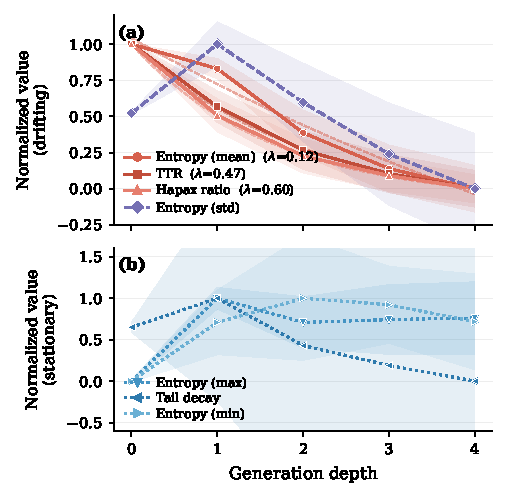
\includegraphics[width=\textwidth]{fig_convergence_dynamics.pdf}
\caption{Feature convergence dynamics. (a)~Drifting features (red) and intermediate entropy std (purple): $|d| > 0.46$ by gen-2+. (b)~Near-stationary features (blue): $|d| < 0.25$ at all depths. Shape stability persists across chain lengths.}
\label{fig:convergence}
\end{figure*}


\section{Discussion}
\label{sec:discussion}

\looseness=-1 DDR reflects monotonic NLL compression under recursive generation (Appendix~\ref{app:nll-distribution}).
Shape stability is not trivially predictable from architecture: entropy\_max is bounded by $\log|V|{\approx}10.8$ nats but observed values fall far below this ceiling; tail\_decay lacks an obvious bound yet remains near-stationary ($|d|{=}0.10$--$0.22$); entropy\_std drifts ($d{=}0.46$) despite shared NLL derivation.
ANOVA confirms depth explains ${>}48{\times}$ more variance in location than shape features (Appendix~\ref{app:variance-decomposition}).

\paragraph{Relationship to model collapse.}
\looseness=-1 Model collapse erodes tail coverage via weight updates, and shape features \emph{do} change under retraining \cite{curse_of_recursion,strong_model_collapse}. DDR, by contrast, characterizes fixed-parameter inference where shape remains stable.
Shape stability is thus specific to the fixed-parameter regime, not an a priori consequence of architecture; DDR complements concurrent iterative-generation studies (Appendix~\ref{app:iterative-comparison}).

\paragraph{Temperature sensitivity.}
\looseness=-1 Higher sampling temperature ($\tau > 0.7$) flattens token probability distributions, narrowing NLL variance and diluting the location shift that drifting features capture (\S\ref{sec:results-differential}).
The DDR partition hierarchy is preserved across all tested temperatures (Appendix~\ref{app:ddr-temp-stability}), but signal strength is temperature-dependent, bounding current applicability to moderate sampling.

\paragraph{Error structure and scope.}
\looseness=-1 The gen-1$\to$gen-2+ boundary is the primary failure point (error rate 48.4\%; Appendix~\ref{app:error-analysis}): gen-1 texts retain sufficient diversity to overlap with gen-0; deeper generations show monotonically decreasing error ($\leq$29.2\%), so DDR-based classifiers are most reliable for heavily recycled content.
The DDR partition is robust across decoding strategies, temperatures, and reference models (Appendices~\ref{app:decoding-strategy}--\ref{app:cross-ref}).
Instruction tuning compresses DDR (Appendix~\ref{app:instruct}), but QLoRA recovery to F1\,=\,0.89--0.91 (within-model) shows the signal persists.
Cross-domain (F1\,=\,0.74--0.75; Appendix~\ref{app:domain}) and 9-generator (Appendix~\ref{app:9gen-scale}) evaluations confirm generalization.
DDR enables corpus contamination detection and synthetic data pipeline auditing; depth-aware filtering does not improve perplexity (Appendix~\ref{app:downstream}), so DDR identifies \emph{provenance} rather than \emph{fluency degradation}. Finer-grained 5-class classification yields F1\,$\approx$\,0.50 (Appendix~\ref{app:finer-depth}), a resolution limit of three depth classes.

\section{Conclusion}
\label{sec:conclusion}

\looseness=-1 Recursive generation produces a decomposable depth response: location features drift monotonically while shape features remain approximately preserved. This asymmetry supports cross-generator depth classification (F1\,=\,0.694--0.762; 5-generator cross-model F1\,=\,0.830) under moderate sampling temperatures ($\tau \leq 0.7$).
Instruction tuning compresses DDR, bounding current applicability to base models; QLoRA recovery (F1\,=\,0.89--0.91, within-model) points to tractable extension to instruct settings.

\section*{Limitations}
\label{sec:limitations}

\looseness=-1 All eight generators are base (pretrained) models with $\leq$8.2B parameters; instruction-tuned variants show substantially degraded depth signal (within-model 3-class F1 drops 3.7--19.9\,pp; Appendix~\ref{app:instruct}), though QLoRA partially recovers (F1\,=\,0.89--0.91, within-model); this pattern is consistent with signal compression rather than elimination.
The evaluation assumes English Wikipedia seeds, a fixed decoding regime ($t{=}0.7$, nucleus $p{=}0.9$), and an English-centric reference model (Pythia-410M); cross-temperature transfer is tested (Appendix~\ref{app:cross-temp}) but cross-lingual generalization remains untested.
Depth resolution is bounded at three classes (gen-0\,/\,gen-1\,/\,gen-2+); finer-grained 5-class classification yields F1\,$\approx$\,0.50 with deeper depths mutually indistinguishable (Appendix~\ref{app:finer-depth}).
DDR signal strength is temperature-dependent; at $\tau{=}0.9$, classification performance degrades substantially ($-$9.3 to $-$26.0\,pp binary F1), and cross-temperature transfer at production scales remains untested.

\section*{Ethics Statement}
\label{sec:ethics}

All texts analyzed in this work are LLM-generated from publicly available Wikipedia seeds; no personal or sensitive data is involved.
Our method estimates the generation depth of a text passage (how many recursive generation steps it has undergone), not the identity of its author.
Individual authorship attribution is outside both the scope and the capability of this approach; privacy implications are minimal.
We acknowledge that depth estimation tools could in principle be used to selectively suppress machine-generated text in contexts where such content is legitimate (e.g., accessibility tools, assistive writing).
We encourage deployment in data governance pipelines where provenance transparency, rather than content removal, is the objective.
All code, data, and trained models will be released upon publication.

\paragraph{Licenses.}
All generator models are publicly available under permissive licenses (Apache 2.0 for Pythia, OLMo, and Mistral; Qwen License for Qwen3; Llama Community License for Llama 3.2).
Wikipedia seed passages are distributed under CC BY-SA 3.0.

\paragraph{Compute budget.}
All experiments were conducted on 4$\times$ NVIDIA RTX 5090 GPUs (32\,GB each), totaling approximately 62 GPU-hours.

\paragraph{Software.}
Experiments used Python 3.12.3, PyTorch 2.10.0 (CUDA 12.8), Transformers 4.57.6, XGBoost 3.2.0, scikit-learn 1.8.0, NumPy 2.2.6, pandas 3.0.2, and SciPy 1.17.1.

\bibliography{references}

\appendix
\renewcommand{\thesection}{\alphalph{\value{section}}}

\noindent\textbf{Note:} Unless otherwise stated, appendix experiments use the original six-generator subset (Pythia-2.8B/1B, OLMo-2-1B, Qwen3-1.7B/0.6B/8B).
Main paper results (\S\ref{sec:results}) use the full eight-generator set (adding Llama-3.2-3B and Mistral-7B-v0.3).

\section{Dataset Statistics}
\label{app:dataset-stats}

Table~\ref{tab:dataset-stats} reports per-generator sample counts after filtering (removing generation failures, exact duplicates, and passages shorter than 50 whitespace tokens).
Under the 3-class evaluation scheme, the dataset contains 7{,}963 gen-0 samples (21.5\%), 7{,}896 gen-1 (21.3\%), and 21{,}199 gen-2+ (57.2\%, combining depths 2--4).
The gen-2+ majority reflects the chain structure (three deeper depths per chain vs.\ one each for gen-0 and gen-1); class-balanced sampling is applied during evaluation.

\begin{table}[t]
\centering
\small
\caption[Per-generator sample counts]{Per-generator sample counts after filtering (8 generators, 5 families). Each generator starts from ${\sim}$1{,}000 shared Wikipedia seeds and produces chains of depth 4 (5 texts per chain). Attrition varies by generator due to differing generation failure rates.\protect\footnotemark}
\label{tab:dataset-stats}
\begin{tabular}{llcc}
\toprule
\textbf{Generator} & \textbf{Family} & \textbf{Params} & \textbf{Samples} \\
\midrule
Pythia-1B       & Pythia  & 1.0B & 4{,}555 \\
Pythia-2.8B     & Pythia  & 2.8B & 4{,}609 \\
OLMo-2-1B      & OLMo    & 1.5B & 4{,}713 \\
Qwen3-0.6B     & Qwen    & 0.6B & 4{,}538 \\
Qwen3-1.7B     & Qwen    & 1.7B & 4{,}617 \\
Qwen3-8B       & Qwen    & 8.2B & 4{,}497 \\
Llama-3.2-3B   & Llama   & 3.2B & 4{,}680 \\
Mistral-7B-v0.3 & Mistral & 7.0B & 4{,}849 \\
\midrule
\multicolumn{3}{l}{\textbf{Total}} & \textbf{37{,}058} \\
\bottomrule
\end{tabular}
\end{table}
\footnotetext{Table~\ref{tab:baselines} evaluates on a subset of 34{,}131 samples for which all detector scores (FastDetectGPT, Binoculars, LD-Score, Avg-LogProb) are available.}

Figure~\ref{fig:violin} shows the full distribution of each feature across five generation depths (0--4), pooled across all eight generators ($N$\,=\,37{,}058).
The violin plots confirm the DDR pattern: drifting features (entropy mean, TTR, hapax ratio) show progressive narrowing and location shift, while shape features (entropy max, tail decay) maintain approximately constant distributions across depths.

\begin{figure*}[!htbp]
\centering
\includegraphics[width=\textwidth]{fig_appendix_violin.pdf}
\caption{Feature distributions by generation depth (violin plots, $N$\,=\,37{,}058). Drifting features (entropy mean, TTR, hapax ratio: $|\rho| > 0.60$) show clear location shifts and narrowing with increasing depth. Shape features (entropy max, tail decay: $|\rho| < 0.10$) remain approximately stationary. Quartile lines indicate median and interquartile range.}
\label{fig:violin}
\end{figure*}


\section{Length Confound Analysis}
\label{app:length}
% Appendix — Length Confound Analysis
% Data source: 8-generator LOGO corpus (37,058 samples)

Surface diversity features (TTR, hapax ratio) mechanically depend on text length:
shorter texts yield higher type-token ratios by construction.
If generation depth systematically shortens text, observed depth trends could be length artifacts rather than genuine distributional shifts.
We investigate with three complementary analyses.

\paragraph{(a) Length--depth correlation.}
Spearman rank correlation between word count and generation depth is weak across all eight generators ($|\rho| < 0.14$); depth does not systematically shorten or lengthen text in our corpus.

\paragraph{(b) Length--feature correlations.}
While length--depth correlation is weak, individual features show moderate length dependence:
tail\_decay ($|\rho| = 0.38$), hapax\_ratio ($|\rho| = 0.30$), and TTR ($|\rho| = 0.29$).
Reference-model features show weaker length correlations (entropy\_mean $|\rho| = 0.09$, entropy\_std $|\rho| = 0.18$).
This motivates the length-matched evaluation below: if length mediates some depth--feature association, controlling for length will reduce classification performance.

\paragraph{(c) Length-matched classification.}
We subsample the dataset so that word-count distributions are equalized across depth classes (gen-0\,/\,gen-1\,/\,gen-2+), then retrain the binary XGBoost classifier under pooled LOGO (8-fold).
Length-matched binary F1\,=\,0.724, down from 0.770 on the unmatched set ($\Delta$\,=\,$-$0.046).
The matched subset is smaller than the full corpus; a random-subsample control at equal $N$ (below) isolates the deconfounding effect from the sample-size reduction.
To distinguish this from a sample-size effect, we run a random-subsample control at equal $N$ without length matching: F1\,=\,0.767, which confirms that the 0.046 drop reflects genuine length deconfounding rather than reduced data.

\paragraph{Conclusion.}
Length accounts for approximately 6\% of discriminative performance ($\Delta$\,=\,0.046 out of 0.770).
The majority of the depth signal is length-independent: length-matched F1 (0.724) remains far above chance and substantially above all individual detection baselines (\S\ref{sec:results-baselines}).
Surface features (TTR, hapax\_ratio) partially co-vary with length, but their depth-discriminative contribution persists after length control, consistent with generation-induced vocabulary compression operating independently of text truncation.


\section{Prompt Type Generalization}
\label{app:prompt-type}
We evaluate depth profiling under three prompt types using Pythia-2.8B. Each uses 995 seeds $\times$ 5 depths. The exact templates are:

\begin{tcolorbox}[colback=yellow!5!white, colframe=gray!50, title=Prompt Templates, breakable, fonttitle=\bfseries\small]
\textbf{Continuation:} \texttt{Continue the following text: \{text\}}\\[4pt]
\textbf{Elaboration:} \texttt{Elaborate on the following text: \{text\}}\\[4pt]
\textbf{Inspired rewriting:} \texttt{Write a new passage inspired by the following text: \{text\}}
\end{tcolorbox}

\paragraph{Within-prompt-type classification.}
5-fold CV macro-F1: continuation 0.78, rewriting 0.74, elaboration 0.73. All three prompt types exhibit the same differential depth response pattern: drifting features (hapax ratio, TTR, entropy mean) show consistent monotonic trends, while near-stationary features (entropy max, tail decay) change by less than 5\%.

\paragraph{Cross-prompt-type transfer (LOPTO).}
Leave-one-prompt-type-out evaluation yields average F1\,=\,0.753, which confirms that depth signal transfers across prompt types. Feature decay rates differ: continuation shows the strongest drift (16.9\% per depth step), followed by rewriting (6.1\%) and elaboration (1.4\%), consistent with continuation chains applying less semantic constraint on the output.

\FloatBarrier

\section{Finer-Grained Depth Classification}
\label{app:finer-depth}
We evaluate finer-grained 5-class depth classification (gen-0 through gen-4) using the same 7-feature ensemble and LOGO protocol described in \S\ref{sec:method}.

\begin{table}[ht]
\centering
\small
\caption{5-class LOGO evaluation. Each row holds out one generator for testing, training on the remaining five.}
\label{tab:5class-logo}
\resizebox{\linewidth}{!}{%
\begin{tabular}{lcccc}
\toprule
\textbf{Held-out Generator} & \textbf{Macro F1} & \textbf{Weighted F1} & \textbf{Accuracy} \\
\midrule
OLMo-2-1B       & 0.484 & 0.506 & 0.524 \\
Pythia-1B        & 0.543 & 0.568 & 0.575 \\
Pythia-2.8B      & 0.523 & 0.540 & 0.560 \\
Qwen3-0.6B      & 0.513 & 0.521 & 0.546 \\
Qwen3-1.7B      & 0.510 & 0.536 & 0.548 \\
Qwen3-8B        & 0.434 & 0.455 & 0.493 \\
\midrule
\textbf{Average} & \textbf{0.501 $\pm$ 0.038} & \textbf{0.521} & \textbf{0.541} \\
\bottomrule
\end{tabular}}
\end{table}

\begin{table}[ht]
\centering
\small
\caption{Per-class F1 averaged across all six LOGO folds.}
\label{tab:5class-perclass}
\resizebox{\linewidth}{!}{%
\begin{tabular}{lccccc}
\toprule
\textbf{Metric} & \textbf{Gen-0} & \textbf{Gen-1} & \textbf{Gen-2} & \textbf{Gen-3} & \textbf{Gen-4} \\
\midrule
Avg F1      & 0.921 & 0.634 & 0.268 & 0.259 & 0.423 \\
\bottomrule
\end{tabular}}
\end{table}

\paragraph{Analysis.}
Moving from 3-class (gen-0 / gen-1 / gen-2+) to 5-class classification reduces LOGO macro F1 to approximately 0.50 (six-generator subset; the 3-class baseline for this subset is comparable to the 8-generator result of 0.762 in Table~\ref{tab:logo-results}).
The degradation is concentrated in the middle depths: gen-2 and gen-3 achieve only 0.268 and 0.259 F1, respectively.
The aggregated confusion matrix reveals that 36.5\% of true gen-2 samples are misclassified as gen-1, while 37.8\% of true gen-3 samples are predicted as gen-4.
Adjacent depths (gen-2$\leftrightarrow$gen-3, gen-3$\leftrightarrow$gen-4) account for the majority of errors, consistent with the intuition that deeper recursive generations converge in surface-level statistical signatures.
Gen-0 (human text) remains highly distinguishable (F1 = 0.921), and gen-1 retains moderate separability (F1 = 0.634).
Shape features that are near-stationary in the 3-class setting become substantially more important under 5-class evaluation: permutation importance of entropy\_std increases by 93\% and tail\_decay by 400\% relative to 3-class, yet these gains are insufficient to resolve adjacent depths.
These results support the 3-class grouping adopted in the main paper: collapsing gen-2+ preserves the most informative boundary (human vs.\ first-generation vs.\ deeper recursion) while avoiding the noise introduced by near-identical adjacent depths.

\paragraph{Classifier comparison.}
To verify that 5-class degradation reflects feature-level limitations rather than classifier choice, we evaluate four alternatives under the same protocol: HistGradientBoosting (macro F1\,=\,0.501, 95\% bootstrap CI [0.496, 0.506]), random forest (0.476), logistic regression (0.447), and Frank-Hall ordinal reduction (0.451).
All classifiers perform comparably to the default XGBoost ensemble (0.501); classifier capacity is not the bottleneck.
The gen-2/gen-3 boundary is the primary failure mode across all methods: these two classes are effectively inseparable with the current feature set. This establishes 3-class granularity as the practical ceiling for surface and entropy features.
At the 3-class level, ordinal-specific methods (CORAL ordinal regression, Frank-Hall reduction) similarly fail to improve over multiclass XGBoost (\S\ref{sec:results}), which confirms that the bottleneck is feature separability across all granularities, not the modeling of label ordinality.

\FloatBarrier

\section{End-to-End Depth Classification (QLoRA)}
\label{app:qlora}
To assess whether depth signal extends beyond handcrafted features, we fine-tune a pretrained language model end-to-end as a depth classifier using QLoRA \cite{qlora}.

\paragraph{Setup.}
We fine-tune Qwen3-0.6B-Base with LoRA rank 16, learning rate $2 \times 10^{-4}$, and 3 epochs, framing depth estimation as 5-class sequence classification (gen-0 through gen-4).\footnote{Evaluated on a 4-generator subset (Pythia-1B, OLMo-2-1B, Qwen3-0.6B, Qwen3-1.7B) using 5-fold stratified CV; XGBoost 3-class F1\,=\,0.805 under the same protocol. We expect 8-generator training to further improve given additional diversity; the comparison direction is preserved.}
For 3-class evaluation, we collapse predictions into gen-0\,/\,gen-1\,/\,gen-2+ post hoc.
All results use 5-fold stratified cross-validation on the 4-generator subset.

\begin{table}[ht]
\centering
\small
\caption{QLoRA end-to-end depth classification vs.\ XGBoost on handcrafted features, under 5-fold stratified CV (4-generator subset).}
\label{tab:qlora}
\resizebox{\linewidth}{!}{%
\begin{tabular}{lccc}
\toprule
\textbf{Method} & \textbf{5-class F1} & \textbf{3-class F1} & \textbf{Per-class F1 (5-class)} \\
\midrule
XGBoost (7 features) & 0.497 $\pm$ 0.008 & 0.805 $\pm$ 0.008 & --- \\
QLoRA (Qwen3-0.6B)   & 0.583 $\pm$ 0.010 & 0.905 $\pm$ 0.003 & 0.999\,/\,0.796\,/\,0.413\,/\,0.259\,/\,0.447 \\
\bottomrule
\end{tabular}}
\end{table}

\paragraph{Results.}
QLoRA achieves 3-class F1\,=\,0.905 ($\pm$0.003) under 5-fold stratified CV on a 4-generator subset, a +10.0\,pp improvement over the same-subset XGBoost baseline (0.805).
On 5-class evaluation, QLoRA reaches F1\,=\,0.583 ($\pm$0.010) vs.\ 0.497 for XGBoost (+8.6\,pp), with the largest gains at gen-1 (0.796 vs.\ 0.650) and gen-2 (0.413 vs.\ 0.267).
The gen-2/gen-3 boundary remains the primary failure mode (gen-3 F1\,=\,0.259), consistent with the feature-level analysis in \S\ref{sec:discussion}.

\paragraph{Hyperparameter robustness.}
A second run with LoRA rank 32 and seed 123 yields 5-class F1\,=\,0.587 ($\pm$0.005) and 3-class F1\,=\,0.905 ($\pm$0.004), which confirms stability across hyperparameter and seed variation ($\Delta < 1$\,pp on both metrics).

\paragraph{Implications.}
The substantial 3-class improvement demonstrates that raw token embeddings contain depth signal beyond what summary statistics capture; the seven handcrafted features are a strong but lossy compression of the full distributional information.
End-to-end fine-tuning exploits token-level patterns (e.g., positional regularities, n-gram repetitions) that aggregate features cannot represent.
This confirms that the depth signal documented in our main analysis is real and exploitable beyond engineered features, while the handcrafted approach retains practical advantages: interpretability, computational efficiency (no GPU inference), and the ability to reveal the differential depth response pattern that motivates the task formulation.
The QLoRA ceiling thus represents an information-asymmetric upper bound rather than a competing method: it consumes the full token sequence (0.6B parameters, GPU inference) whereas the 7-feature ensemble distills the signal into interpretable scalars that expose \emph{why} depth is detectable, a decomposition that end-to-end models cannot provide.

\FloatBarrier

\section{Leave-One-Feature-Out Analysis}
\label{app:lofo}
\looseness=-1 We complement the permutation importance analysis (\S\ref{sec:results-differential}) with a leave-one-feature-out ablation. Each row drops one of the seven features and re-evaluates the full 6-gen LOGO protocol; $\Delta$ is the change relative to the full 7-feature ensemble (F1\,=\,0.789).

\begin{table}[ht]
\centering
\small
\caption{Leave-one-feature-out ablation (6-gen LOGO). Each row drops one feature and re-evaluates with the LOGO protocol. Sorted by impact magnitude.}
\label{tab:lofo}
\begin{tabular}{lcc}
\toprule
\textbf{Dropped feature} & \textbf{LOGO F1} & $\boldsymbol{\Delta}$ \textbf{vs Full} \\
\midrule
entropy\_max    & 0.774 & $-$1.50\,pp \\
entropy\_mean   & 0.783 & $-$0.63\,pp \\
ttr             & 0.784 & $-$0.55\,pp \\
hapax\_ratio    & 0.785 & $-$0.42\,pp \\
tail\_decay     & 0.786 & $-$0.33\,pp \\
entropy\_std    & 0.786 & $-$0.29\,pp \\
entropy\_min    & 0.789 & $+$0.01\,pp \\
\midrule
Full (7 features) & 0.789 & --- \\
\bottomrule
\end{tabular}
\end{table}

\paragraph{Analysis.}
\looseness=-1 Entropy\_max causes the largest degradation when removed ($-$1.5\,pp), despite ranking only fourth in permutation importance (split frequency 0.063). This indicates that entropy\_max provides unique signal (capturing the most surprising token under the reference model) that is not redundant with other features.
Conversely, entropy\_min is fully redundant ($\Delta$\,=\,+0.01\,pp), consistent with its near-zero permutation importance (0.015).
Six of seven features contribute positively to the ensemble, which confirms that the 7-feature design is not over-specified.

\looseness=-1 To verify that feature importance generalizes beyond the original 6-generator subset, we repeat the LOFO analysis on the full 8-generator set (37,058 samples, 10-fold stratified CV). Table~\ref{tab:lofo-8gen} confirms consistent rankings: \texttt{entropy\_max} remains the most impactful feature ($\Delta=-0.019$), followed by \texttt{entropy\_mean} ($\Delta=-0.012$). All seven features contribute positively, with no feature becoming redundant upon dataset expansion.

\paragraph{Minimal sufficient subset.}
\looseness=-1 To assess feature redundancy, we evaluate all $\binom{7}{2}{=}21$ two-feature subsets under 10-fold stratified CV (8-gen, 3-class).
The best pair is \{entropy\_mean, entropy\_max\}, achieving F1\,=\,0.68 (one drifting and one stationary feature), which captures 88\% of the full-ensemble performance (0.771) and confirms that the DDR partition's two components are individually informative.
Adding the remaining five features yields +9.1\,pp; the full set provides meaningful complementarity beyond the minimal core. Nevertheless, the two-feature result demonstrates that the depth signal is not an artifact of feature-set size.

\begin{table}[ht]
\centering
\small
\caption{Leave-one-feature-out importance on the full 8-generator set (37,058 samples). Ranking is consistent with the 6-generator subset (Table~\ref{tab:lofo}).}
\label{tab:lofo-8gen}
\begin{tabular}{lcc}
\toprule
\textbf{Configuration} & \textbf{3-class F1} & $\boldsymbol{\Delta}$ \\
\midrule
Full (7 features) & 0.771 & --- \\
\midrule
$-$ entropy\_max    & 0.752 & $-$0.019 \\
$-$ entropy\_mean   & 0.759 & $-$0.012 \\
$-$ entropy\_std    & 0.763 & $-$0.007 \\
$-$ ttr             & 0.764 & $-$0.007 \\
$-$ hapax\_ratio    & 0.765 & $-$0.005 \\
$-$ entropy\_min    & 0.766 & $-$0.005 \\
$-$ tail\_decay     & 0.767 & $-$0.004 \\
\bottomrule
\end{tabular}
\end{table}

\FloatBarrier

\subsection{Candidate Feature Screening}
\label{app:feature-candidate}
To verify that the seven retained features are not an arbitrary subset, we screened six additional NLL-distributional statistics as candidate features: median, 90th percentile (p90), interquartile range (IQR), coefficient of variation (CV), skewness, and kurtosis.
Table~\ref{tab:candidate-features} reports their DDR coordinates, classification impact, and correlation with retained features.

\begin{table}[ht]
\centering
\small
\caption{Candidate feature screening. All six candidates fall in the drifting DDR zone and correlate strongly ($|r| > 0.65$) with existing features. Adding any combination to the baseline degrades or leaves unchanged LOGO 3-class F1; LOFO $\Delta > 0$ indicates that removing the candidate \emph{improves} classification.}
\label{tab:candidate-features}
\resizebox{\linewidth}{!}{%
\begin{tabular}{lccccl}
\toprule
\textbf{Candidate} & $|\rho|$ & $d$ & \textbf{LOFO} $\Delta$\textbf{F1} & $|r|_{\max}$ & \textbf{Most correlated} \\
\midrule
median    & 0.685 & 0.794 & $+$0.008 & 0.960 & entropy\_mean \\
p90       & 0.693 & 0.960 & $+$0.000 & 0.937 & entropy\_mean \\
IQR       & 0.708 & 1.079 & $+$0.007 & 0.908 & entropy\_std \\
CV        & 0.633 & 0.980 & $-$0.000 & 0.761 & entropy\_mean \\
skewness  & 0.651 & 0.940 & $+$0.010 & 0.780 & entropy\_mean \\
kurtosis  & 0.635 & 0.769 & $-$0.003 & 0.650 & entropy\_mean \\
\bottomrule
\end{tabular}}
\end{table}

\looseness=-1 All six candidates occupy the drifting zone ($|\rho| > 0.63$, $d > 0.77$), overlapping with entropy mean, TTR, and hapax ratio; none introduces a new axis of depth-dependent variation.
Three candidates (median, $r{=}0.96$; p90, $r{=}0.94$; IQR, $r{=}0.91$) are near-perfect linear proxies of existing features.
Adding all six to the 6-feature baseline\footnote{Tail decay requires full-vocabulary logits unavailable in the token-NLL subset used for this analysis; we report 6-feature baselines for fair comparison.} reduces 3-class LOGO F1 from 0.733 to 0.722, consistent with overfitting from redundant inputs.
LOFO analysis on the extended 12-feature set confirms that removing skewness ($+$0.010), median ($+$0.008), or IQR ($+$0.007) \emph{improves} classification; these features inject noise rather than signal.
The retained seven features span three complementary DDR zones (drifting, intermediate, near-stationary) and two modalities (reference-model NLL, surface lexical diversity); additional distributional statistics provide no incremental information.

\FloatBarrier

\section{Confusion Matrix}
\label{app:confusion}
Table~\ref{tab:confusion} reports the aggregated confusion matrix from the original six-generator subset (Pythia-2.8B, Pythia-1B, OLMo-2-1B, Qwen3-1.7B, Qwen3-0.6B, Qwen3-8B) under leave-one-generator-out (LOGO) evaluation, collapsed to three ordinal classes: gen-0 (human), gen-1 (first-generation), and gen-2+ (depth $\geq$ 2).
The later-added Llama-3.2-3B and Mistral-7B-v0.3 are evaluated in the full 8-generator LOGO results (Table~\ref{tab:logo-results}).

\begin{table}[ht]
\centering
\small
\caption{Aggregated 3-class confusion matrix from 6-generator LOGO evaluation ($N=27{,}529$). Each cell shows count and row-normalized percentage. Gen-0 is near-perfectly identified. Gen-1 errors are asymmetric: misclassification as gen-2+ (18.8\%) is 3$\times$ more frequent than as gen-0 (6.2\%). Gen-1 text already carries detectable recursive distortion.}
\label{tab:confusion}
\resizebox{\linewidth}{!}{%
\begin{tabular}{lccc}
\toprule
& \textbf{Pred gen-0} & \textbf{Pred gen-1} & \textbf{Pred gen-2+} \\
\midrule
\textbf{True gen-0} & 5{,}937 (99.4\%) & 35 (0.6\%) & 0 (0.0\%) \\
\textbf{True gen-1} & 368 (6.2\%) & 4{,}437 (75.0\%) & 1{,}113 (18.8\%) \\
\textbf{True gen-2+} & 464 (3.0\%) & 3{,}646 (23.3\%) & 11{,}529 (73.7\%) \\
\bottomrule
\end{tabular}}
\end{table}

Figure~\ref{fig:confusion-heatmap} provides a heatmap visualization of the confusion matrix.
The row-normalized view highlights near-perfect gen-0 classification (99.4\% recall), gen-1 confusion primarily with gen-2+ (18.8\%) rather than gen-0 (6.2\%), and gen-2+ misclassification predominantly into gen-1 (23.3\%), consistent with DDR predictions.

\begin{figure}[H]
\centering
\includegraphics[width=\columnwidth, trim=0 0 344pt 0, clip]{fig_appendix_confusion.pdf}\\[-2pt]
{\small (a) Raw counts}
\caption{3-class LOGO confusion matrix ($N$\,=\,27{,}529). Gen-0 achieves near-perfect classification; the primary confusion axis is gen-1 $\leftrightarrow$ gen-2+.}
\label{fig:confusion-heatmap}
\end{figure}

\begin{figure}[H]
\addtocounter{figure}{-1}
\centering
\includegraphics[width=\columnwidth, trim=344pt 0 0 0, clip]{fig_appendix_confusion.pdf}\\[-2pt]
{\small (b) Row-normalized recall percentages}
\caption{(Continued) Row-normalized view of the confusion matrix.}
\end{figure}

\FloatBarrier

\section{Classifier Sensitivity}
\label{app:classifier}
\looseness=-1 To verify that the depth signal resides in the features rather than the classifier,
we repeat the 6-generator LOGO evaluation using Logistic Regression and Random Forest
in place of XGBoost (Table~\ref{tab:alt-classifier}).
All other settings (the same 7 features, 3-class labels, and class-balanced downsampling) are
kept identical. For Logistic Regression we apply standard scaling to the features.

\begin{table}[ht]
\centering
\caption{LOGO macro-F1 across three classifiers. Each column shows the held-out generator F1. (6-generator LOGO; 3-class.)}
\label{tab:alt-classifier}
\small
\resizebox{\linewidth}{!}{%
\begin{tabular}{lc cccccc}
\toprule
Classifier & Avg F1 & OLMo-2 & Py-1B & Py-2.8B & Qw-0.6B & Qw-1.7B & Qw-8B \\
\midrule
XGBoost          & 0.789 & 0.764 & 0.856 & 0.804 & 0.824 & 0.806 & 0.683 \\
Random Forest    & 0.790 & 0.764 & 0.856 & 0.804 & 0.825 & 0.807 & 0.684 \\
Logistic Regr.   & 0.725 & 0.719 & 0.781 & 0.740 & 0.745 & 0.743 & 0.624 \\
\bottomrule
\end{tabular}}
\end{table}

\looseness=-1 Both tree-based classifiers achieve LOGO F1 $\approx 0.79$,
and even a linear model reaches $0.725$, well above the $0.33$ chance baseline for
three classes.
The per-generator ranking is also consistent across classifiers
(Pythia-1B easiest, Qwen3-8B hardest),
confirming that discriminative power originates in the entropy and lexical features,
not in classifier capacity.
Ordinal-specific methods (CORAL \cite{coral_ordinal}, Frank-Hall \cite{frank_hall_ordinal}) achieve comparable F1 with overlapping CIs, which confirms that 3-class granularity provides insufficient resolution for ranking-aware losses to improve over standard multiclass classification.

\paragraph{XGBoost hyperparameter sensitivity.}
To verify that performance is not an artifact of hyperparameter selection, we vary \texttt{max\_depth} $\in \{3, 4, 6, 8\}$ while keeping all other settings fixed (Table~\ref{tab:xgb-sensitivity}).

\begin{table}[ht]
\centering
\small
\caption{XGBoost \texttt{max\_depth} sensitivity (8-gen LOGO). 3-class F1 varies by only 2.0\,pp; binary F1 (gen-1 vs.\ gen-2+) is effectively invariant ($\leq$0.1\,pp).}
\label{tab:xgb-sensitivity}
\begin{tabular}{lcc}
\toprule
\textbf{max\_depth} & \textbf{3-class F1} & \textbf{Binary F1} \\
\midrule
3 & 0.752 & 0.700 \\
4 & 0.759 & 0.699 \\
6 & 0.769 & 0.700 \\
8 & 0.772 & 0.699 \\
\bottomrule
\end{tabular}
\end{table}

\looseness=-1 3-class F1 increases monotonically with tree depth but the total range is only 2.0\,pp (0.752--0.772); binary F1 is effectively invariant (0.699--0.700).
The default \texttt{max\_depth}\,=\,6 used throughout the paper lies within 0.3\,pp of the best 3-class setting; the reported results are not sensitive to this choice.

\begin{figure}[t]
\centering
\includegraphics[width=\columnwidth]{fig_appendix_confusion.pdf}
\caption{3-class LOGO confusion matrix ($N$\,=\,27{,}529). (a)~Raw counts. (b)~Row-normalized recall percentages. Gen-0 achieves near-perfect classification; the primary confusion axis is gen-1 $\leftrightarrow$ gen-2+.}
\label{fig:confusion-heatmap}
\end{figure}

\subsection*{Sampling Sensitivity Analysis}
\label{app:sampling-sensitivity}

\looseness=-1 To assess robustness to decoding temperature, we regenerate continuation chains at $t \in \{0.5, 0.9\}$ with fixed nucleus $p{=}0.9$ (matching the default) for four generators spanning three model families: Pythia-2.8B, OLMo-2-1B, Qwen3-1.7B, and Qwen3-0.6B (Table~\ref{tab:sampling-ablation}).

\begin{table}[ht]
\centering
\caption{Depth classification under varying temperature (fixed top-$p$\,=\,0.9). Binary: gen-1 vs.\ gen-2+. LOGO evaluation; 95\% bootstrap CIs.$^{\ast}$$^{\dagger}$}
\label{tab:sampling-ablation}
\small
\resizebox{\linewidth}{!}{%
\begin{tabular}{llcc c}
\toprule
Model & Temp & LOGO Binary F1 & 95\% CI & $\rho$(ent.\ mean) \\
\midrule
Pythia-2.8B$^{\dagger}$ & 0.5  & \textbf{0.814} & [.798, .828] & $-0.58$ \\
Pythia-2.8B$^{\dagger}$ & 0.7  & 0.740 & [.725, .755] & $-0.60$ \\
Pythia-2.8B$^{\dagger}$ & 0.9  & 0.480 & [.465, .498] & $-0.30$ \\
\midrule
OLMo-2-1B & 0.5  & \textbf{0.783} & [.768, .798] & $-0.72$ \\
OLMo-2-1B & 0.7  & 0.695 & [.679, .711] & $-0.60$ \\
OLMo-2-1B & 0.9  & 0.453 & [.437, .469] & $-0.26$ \\
\midrule
Qwen3-1.7B$^{\dagger}$ & 0.5  & 0.751 & --- & $-0.60$ \\
Qwen3-1.7B$^{\dagger}$ & 0.7  & 0.751 & --- & $-0.60$ \\
Qwen3-1.7B$^{\dagger}$ & 0.9  & 0.566 & --- & $-0.37$ \\
\midrule
Qwen3-0.6B & 0.5  & 0.711 & [.694, .729] & $-0.67$ \\
Qwen3-0.6B & 0.7  & 0.691 & [.673, .709] & $-0.60$ \\
Qwen3-0.6B & 0.9  & 0.598 & [.582, .615] & $-0.29$ \\
\bottomrule
\end{tabular}}
\end{table}
\noindent\begin{minipage}{\columnwidth}
\scriptsize $^{\ast}$OLMo temperature experiments use OLMo-2-0425-1B; the original OLMo-2-1B-hf weights are no longer publicly available.\par\vspace{1pt}
$^{\dagger}$Pythia-2.8B and Qwen3-1.7B use 6-generator LOGO (pre-expansion); OLMo-2-1B and Qwen3-0.6B use 8-generator LOGO. Within-model comparisons are unaffected.
\end{minipage}\vspace{4pt}

\looseness=-1 Temperature sensitivity is asymmetric and model-dependent. High-temperature degradation ($t{=}0.9$) is universal: all four generators lose $9.3$--$26.0$\,pp in binary F1, with entropy mean's $|\rho|$ weakening to $0.26$--$0.37$ (vs.\ $0.58$--$0.72$ at $t{=}0.5$). Low-temperature improvement ($t{=}0.5$) is model-dependent: Pythia-2.8B and OLMo-2-1B gain $+7.4$ and $+8.8$\,pp respectively, while both Qwen models show negligible change ($0$--$2.0$\,pp). This split tracks model family rather than scale: Qwen3-0.6B (smallest) and Qwen3-1.7B both plateau, while OLMo-2-1B (similar scale to Qwen3-1.7B) benefits substantially. One possible explanation is that Qwen models produce more peaked output distributions at $t{=}0.7$, leaving less room for low-temperature compression to sharpen the depth signal.

\looseness=-1 The method operates reliably within $t \in [0.5, 0.7]$ across all tested models. Degradation onset at $t{=}0.9$ defines the practical upper bound, consistent with the hypothesis that elevated temperature injects sufficient randomness to flatten the distributional drift that DDR exploits (\S\ref{sec:discussion}).

\subsection*{Per-Generator Performance}

Figure~\ref{fig:per-gen} visualizes per-generator LOGO performance.
Pythia models (1B, 2.8B) achieve highest F1, while larger models (Mistral-7B, Qwen3-8B) show degradation.
The scale effect (larger models $\rightarrow$ lower F1) is consistent with higher-capacity models generating text statistically closer to human writing.

\begin{figure*}[t]
\centering
\includegraphics[width=\textwidth]{fig_appendix_per_gen.pdf}
\caption{Per-generator LOGO performance. (a)~Binary and 3-class F1, sorted by binary F1. Dashed lines: pool average. (b)~6-generator LOGO detail heatmap across model families.}
\label{fig:per-gen}
\end{figure*}

\FloatBarrier

\section{Robustness to Text Perturbation}
\label{app:human-edit}
We assess robustness to post-generation text modification by randomly replacing words at varying rates and re-evaluating the 8-generator LOGO pipeline (Table~\ref{tab:human-edit}).
Random word replacement represents a worst-case perturbation: real human editing preserves semantic coherence, so practical degradation is expected to be substantially lower than these estimates.

\begin{table}[ht]
\centering
\small
\caption{Robustness to random word replacement under 8-gen LOGO evaluation (binary: gen-1 vs.\ gen-2+). Bootstrap 95\% CIs on binary F1 ($n$\,=\,1000).}
\label{tab:human-edit}
\resizebox{\linewidth}{!}{%
\begin{tabular}{lccc}
\toprule
\textbf{Perturbation rate} & \textbf{Binary F1} & \textbf{95\% CI} & \textbf{3-class F1} \\
\midrule
0\% (baseline) & 0.695 & [0.680, 0.710] & 0.737 \\
5\%            & 0.650 & [0.635, 0.666] & 0.641 \\
10\%           & 0.614 & [0.599, 0.629] & 0.492 \\
20\%           & 0.591 & [0.576, 0.605] & 0.367 \\
\bottomrule
\end{tabular}}
\end{table}

Binary depth discrimination (gen-1 vs.\ gen-2+) degrades sublinearly: the first 5\% replacement causes the largest drop ($-$4.6\,pp), with diminishing marginal impact thereafter ($-$3.6\,pp for 5\%$\to$10\%, $-$2.3\,pp for 10\%$\to$20\%).
At 10\% replacement, binary F1 remains 0.614, well above the 0.50 random baseline, which indicates that depth signal survives moderate perturbation.

Three-class classification is more sensitive (0.737$\to$0.367 at 20\%), because distinguishing gen-0 from gen-1 relies heavily on lexical diversity features (TTR, hapax ratio) that are directly disrupted by word replacement.
The binary metric, which excludes gen-0, is inherently more robust since it depends primarily on reference-model entropy features distributed across many tokens.

\paragraph{Feature subset degradation.}
Table~\ref{tab:feature-degrade} compares perturbation robustness of the full 7-feature ensemble against an entropy-only subset (5 reference-model features).
The higher unperturbed binary F1 of the entropy-only subset (0.833 vs.\ 0.695) reflects the strong discriminability of reference-model features for the coarse binary task (gen-1 vs.\ gen-2+); however, lexical features are essential for the finer-grained ordinal task (3-class F1: 0.737 vs.\ 0.688) and provide greater robustness under perturbation.
At 20\% replacement, the 7-feature ensemble surpasses entropy-only on binary F1 (0.591 vs.\ 0.566), despite starting from a lower baseline.
Random word replacement drastically alters per-token context and makes entropy features (computed over the full token sequence) extremely sensitive to noise.
Lexical features (TTR, hapax ratio), as document-level summary statistics, are more stable under per-word perturbation and act as stabilizers in the full ensemble.
The crossover confirms that degradation in the full feature set reflects genuine signal disruption rather than a lexical-feature artifact.

\begin{table}[ht]
\centering
\small
\caption{Feature subset degradation under random word replacement (8-gen LOGO). Entropy-only: 5 reference-model features; 7-feature: full ensemble including lexical features.}
\label{tab:feature-degrade}
\resizebox{\linewidth}{!}{%
\begin{tabular}{lcccc}
\toprule
\textbf{Perturb.} & \textbf{Ent-only Bin} & \textbf{7-feat Bin} & \textbf{Ent-only 3-cl} & \textbf{7-feat 3-cl} \\
\midrule
0\%  & 0.833 & 0.695 & 0.688 & 0.737 \\
5\%  & 0.736 & 0.650 & 0.539 & 0.641 \\
10\% & 0.657 & 0.614 & 0.427 & 0.492 \\
20\% & 0.566 & 0.591 & 0.314 & 0.367 \\
\bottomrule
\end{tabular}}
\end{table}

\paragraph{Baseline comparison.}
Table~\ref{tab:baseline-robustness} compares robustness across detection methods under identical perturbation conditions (8-gen LOGO, binary: gen-1 vs.\ gen-2+).

\begin{table}[ht]
\centering
\small
\caption{Baseline robustness under random word replacement (8-gen LOGO, binary F1). Bold indicates highest F1 at each perturbation rate. (Baseline scores use default XGBoost settings; trends are consistent with the unified configuration in Table~\ref{tab:baselines}.)}
\label{tab:baseline-robustness}
\begin{tabular}{lcccc}
\toprule
\textbf{Method} & \textbf{0\%} & \textbf{5\%} & \textbf{10\%} & \textbf{20\%} \\
\midrule
7-feature ensemble & \textbf{0.695} & 0.650 & 0.614 & 0.591 \\
LD-Score           & 0.677 & \textbf{0.673} & \textbf{0.677} & \textbf{0.671} \\
Avg-LogProb        & 0.682 & 0.419 & 0.335 & 0.375 \\
FastDetectGPT      & 0.571 & 0.437 & 0.468 & 0.514 \\
Binoculars\textsuperscript{\dag}         & 0.500 & 0.461 & 0.446 & 0.425 \\
\bottomrule
\end{tabular}

\vspace{2pt}
{\footnotesize \textsuperscript{\dag}Binoculars operates at chance level on this binary task; its degradation figures are not meaningful.}
\end{table}

The 7-feature ensemble achieves the highest unperturbed binary F1 (0.695), but LD-Score surpasses it under perturbation due to near-zero degradation ($-$0.6\,pp across the full 0\%$\to$20\% range).
FastDetectGPT and Avg-LogProb exhibit non-monotonic degradation at higher perturbation rates, likely because severe perturbation introduces distributional artifacts that these token-level methods detect as anomalous.
Avg-LogProb is the most fragile overall ($-$34.7\,pp at 10\%), while FastDetectGPT drops sharply at 5\% ($-$13.4\,pp) before partially recovering.
LD-Score is nearly invariant to perturbation, consistent with its reliance on corpus-level distributional divergence rather than per-token likelihoods.
The 7-feature ensemble offers the highest starting performance among single-reference methods, with sublinear degradation ($-$10.4\,pp at 20\%).

\paragraph{LLM-simulated sentence regeneration.}
To test robustness under semantically coherent editing, we use Qwen3-0.6B-Base to randomly regenerate 1--3 sentences per passage (avg 1.69 sentences, ${\sim}$50\% edit distance) and re-evaluate the 8-gen LOGO pipeline.
Binary F1 drops from 0.692 to 0.647 ($-$4.5\,pp, 6.5\% relative); 3-class F1 drops from 0.739 to 0.667 ($-$7.1\,pp, 9.7\% relative).
The binary degradation ($-$4.5\,pp) is nearly identical to that caused by 5\% random word replacement ($-$4.6\,pp), despite the LLM rephrase altering ${\sim}$50\% of characters.
This asymmetry arises because LLM-generated replacements preserve the underlying statistical signature of the generation process (entropy dynamics, depth-accumulated distributional drift), whereas random word substitution directly destroys local statistical signals.
Depth profiling thus captures deep generative structure that survives semantic-preserving edits.

\paragraph{Seed complexity.}
Performance is stable across seed text complexity: stratifying seeds by vocabulary richness (TTR terciles) yields maximum F1 variation of 1.1\,pp across groups.

\FloatBarrier

\section{Cross-Domain Generalization}
\label{app:domain}
This pilot study evaluates whether depth signal generalizes beyond Wikipedia by constructing generation chains from three additional domains: News articles, Academic abstracts, and Code documentation.
For each domain, we sample 200 seed texts and generate chains of depth 3 using three generators (Pythia-1B, Qwen3-1.7B, Mistral-7B).
The same 7-feature ensemble and LOGO protocol are applied.

\noindent\textbf{Important caveat:} Cross-domain generation used $t{=}1.0$, top-$p{=}1.0$, which falls outside the method's reliable operating range ($t \leq 0.7$; Appendix~\ref{app:sampling-sensitivity}). Domain and temperature effects are therefore confounded in the results below; the cross-domain signal may partly reflect temperature-induced distributional divergence rather than domain generalization alone.

\begin{table}[ht]
\centering
\small
\caption{Cross-domain depth classification under LOGO evaluation (binary: gen-1 vs.\ gen-2+). Three generators $\times$ 200 seeds per domain. Bootstrap 95\% CIs ($n$\,=\,1000).}
\label{tab:domain}
\begin{tabular}{lccc}
\toprule
\textbf{Domain} & \textbf{Binary F1} & \textbf{95\% CI} & \textbf{3-class F1} \\
\midrule
Code           & 0.754 & [0.737, 0.770] & 0.634 \\
News           & 0.746 & [0.726, 0.764] & 0.652 \\
Academic       & 0.739 & [0.720, 0.757] & 0.622 \\
\bottomrule
\end{tabular}
\end{table}

All three non-Wikipedia domains achieve binary F1 $>$ 0.73 under leave-one-generator-out evaluation. Depth signal is not an artifact of Wikipedia text properties.
The Code-domain 3-class F1 (0.634) likely reflects domain mismatch in the Wikipedia-trained reference model (Pythia-410M), whose NLL estimates may be less discriminative for code syntax; these cross-domain results are preliminary.

\paragraph{Domain $\times$ temperature interaction.}
Cross-domain generation used $t{=}1.0$, top-$p{=}1.0$ (vs.\ the main experiment's $t{=}0.7$, top-$p{=}0.9$).
Supplementary evaluation at $t{=}0.7$ reveals a domain $\times$ temperature interaction: the main Wikipedia experiment favors lower temperature (depth signal degrades monotonically with rising temperature; Appendix~\ref{app:sampling-sensitivity}), while cross-domain evaluation favors higher temperature ($t{=}1.0$ yields +3 to +11\,pp over $t{=}0.7$; News 0.746 vs.\ 0.712, Academic 0.739 vs.\ 0.628, Code 0.754 vs.\ 0.687).
This asymmetry likely reflects reference-model calibration: Pythia-410M, trained predominantly on web text, detects subtle per-step drift in Wikipedia but requires larger distributional divergence (produced by higher temperature) to detect depth signal in out-of-distribution domains.
This finding suggests that reference model selection is a key factor for cross-domain deployment of depth profiling.

\paragraph{3-class inversion as DDR evidence.}
In the cross-domain setting, 3-class F1 (0.62--0.65) falls below binary F1 (0.74--0.75), reversing the pattern observed in the main experiment (3-class 0.762 $>$ binary 0.694).
This inversion reflects degraded gen-0 vs.\ gen-1 separation: the Pythia-410M reference model is calibrated to Wikipedia text, so its baseline entropy estimates are less discriminative for out-of-domain human text and compresses the feature distance between gen-0 and gen-1.
The binary task (gen-1 vs.\ gen-2+) is unaffected because both classes are generated under identical domain and decoding conditions; recursive drift is a relative change that does not depend on absolute calibration.
This pattern provides additional evidence that DDR captures base-model generation dynamics rather than domain-specific text properties: depth signal remains robust even when the human-vs-machine boundary becomes less distinct.

\FloatBarrier

\section{Instruction-Tuned Model Analysis}
\label{app:instruct}
\subsection*{Instruction-Tuned Model Results}

Table~\ref{tab:instruct} summarizes depth classification under instruction tuning for three model families.
All results use within-model 5-fold CV on single-generator chains; LOGO evaluation is available for two models but uses earlier generator subsets (5--6 generators), so cross-model numbers are not directly comparable across rows.

\begin{table}[ht]
\centering
\small
\caption{Depth classification: base vs.\ instruction-tuned models (within-model 5-fold CV). $\rho$: Spearman correlation of entropy mean with depth. Rev.: number of features (out of 7) whose $\rho$ reverses sign under instruction tuning.}
\label{tab:instruct}
\resizebox{\linewidth}{!}{%
\begin{tabular}{lcc cc cc c}
\toprule
& \multicolumn{2}{c}{\textbf{3-class F1}} & \multicolumn{2}{c}{\textbf{Binary F1}} & \multicolumn{2}{c}{$\boldsymbol{\rho}$\textbf{(ent.\ mean)}} & \\
\cmidrule(lr){2-3} \cmidrule(lr){4-5} \cmidrule(lr){6-7}
\textbf{Model} & Base & Instruct & Base & Instruct & Base & Instruct & \textbf{Rev.} \\
\midrule
OLMo-2-1B       & 0.754 & 0.575 & 0.845 & 0.813 & $-$0.64 & $+$0.48 & 6/7 \\
Qwen3-1.7B      & 0.769 & 0.732 & 0.861 & 0.875 & $-$0.60 & $+$0.48 & 6/7 \\
Llama-3.2-3B    & 0.742 & 0.544 & 0.849 & 0.838 & $-$0.63 & $+$0.23 & 3/7 \\
\bottomrule
\end{tabular}}
\end{table}

Instruction tuning degrades 3-class F1 by 3.7--19.9\,pp across all three families, while binary F1 (gen-1 vs.\ gen-2+) changes remain small ($|\Delta| \leq 3.2$\,pp).
The asymmetry indicates that instruction tuning primarily disrupts the gen-0/gen-1 boundary (human vs.\ first-generation), consistent with RLHF shifting the output distribution away from human-like text.
Entropy-mean $\rho$ reverses sign for all three models ($-0.60$--$-0.64$ base $\rightarrow$ $+0.23$--$+0.48$ instruct), and 6 of 7 features reverse for OLMo and Qwen vs.\ 3 of 7 for Llama.
This pattern is consistent with instruction tuning shifting the generation attractor rather than eliminating iterative dynamics (\S\ref{sec:discussion}).

\paragraph{Retraining on instruction-tuned data.}
To test whether the depth signal persists under instruction tuning with reversed polarity, we retrain the XGBoost classifier on instruction-tuned feature data (Table~\ref{tab:instruct-retrain}).

\begin{table}[ht]
\centering
\small
\caption{Classification recovery under instruction-tuned retraining (binary-only: gen-1 vs.\ gen-2+, gen-0 excluded from training and evaluation). Base$\rightarrow$Inst: base-trained classifier tested on instruct data. Note: Table~\ref{tab:instruct} reports higher instruct binary F1 (e.g., OLMo 0.813) because it uses 3-class training with binary evaluation, where gen-0 in training helps the classifier learn the feature space.}
\label{tab:instruct-retrain}
\begin{tabular}{lccc}
\toprule
\textbf{Model} & \textbf{Base$\rightarrow$Inst} & \textbf{Retrained} & \textbf{$\Delta$} \\
\midrule
OLMo-2-1B-Inst   & 0.321 & 0.590 & $+$0.269 \\
Qwen3-1.7B-Inst  & 0.500 & 0.660 & $+$0.160 \\
Qwen3-0.6B-Inst  & 0.532 & 0.600 & $+$0.068 \\
\bottomrule
\end{tabular}
\end{table}

Retraining recovers substantial within-model performance ($+$6.8--26.9\,pp), but the retrained F1 (0.590--0.660) remains below base-model levels (0.69--0.72). Instruction tuning compresses depth signal beyond what retraining on reversed-polarity features can fully recover.

\paragraph{DDR structure under instruction tuning.}
$k{=}2$ clustering in $(|\rho|, d)$ space on pooled instruct features yields silhouette\,=\,0.372 (vs.\ 0.660 for base models); the clean drifting/non-drifting partition is substantially compressed.
The compression is model-dependent: OLMo-Instruct shows near-zero $|\rho|$ for TTR and hapax (0.006, 0.025), while Qwen instruct models retain moderate correlations ($|\rho|{=}0.48$--$0.53$).
Cross-condition transfer is near chance in both directions (base$\rightarrow$instruct binary F1\,=\,0.490; instruct$\rightarrow$base F1\,=\,0.454), with the asymmetry ($-$0.036) suggesting that instruct-trained features generalize even less to base distributions than the reverse.
These results indicate that instruction tuning compresses the feature-space structure underlying DDR rather than simply reversing feature directions (Figure~\ref{fig:instruct-ddr}).

\begin{figure}[t]
\centering
\includegraphics[width=\columnwidth]{fig_appendix_instruct_ddr.pdf}
\caption{DDR partition under base vs.\ instruction-tuned models. (a)~Base models (silhouette\,=\,0.660): clear drifting/non-drifting separation. (b)~Instruction-tuned models (silhouette\,=\,0.372): all features compress toward zero, collapsing the partition; entropy max shifts from near-stationary to intermediate; formerly drifting features (hapax, TTR) lose most of their effect size. Bars show pooled $|d|$; markers show individual generators.}
\label{fig:instruct-ddr}
\end{figure}

\paragraph{Reference model sensitivity.}
One hypothesis for the instruct degradation is reference-model mismatch: the base Pythia-410M reference may produce systematically biased NLL estimates on instruction-tuned outputs, masking depth-dependent variation.
To test this, we replace the reference with Qwen3-0.6B-Instruct and recompute all features on the two instruct generators.
The hypothesis is partially rejected: Qwen3-1.7B-Instruct shows mixed changes (entropy max $d$: $0.51 \to 0.08$, becoming near-stationary; entropy std $d$: $1.07 \to 1.51$, increasing), while OLMo-Instruct loses nearly all depth signal (entropy mean $d$: $1.33 \to 0.02$; tail decay $d$: $0.60 \to 0.06$).
The model-dependent heterogeneity rules out reference mismatch as a universal explanation for instruct DDR degradation. Alignment fundamentally reshapes the generation dynamics rather than introducing a correctable measurement artifact.

\paragraph{End-to-end instruct classification.}
To test whether depth signal persists at the token level despite summary-statistic degradation, we apply the QLoRA end-to-end classifier (Appendix~\ref{app:qlora}) to instruction-tuned data using within-model 5-fold stratified CV (Table~\ref{tab:instruct-qlora}).

\begin{table}[ht]
\centering
\small
\caption{End-to-end QLoRA vs.\ XGBoost on instruction-tuned data (within-model 5-fold CV, Qwen3-0.6B backbone). Base QLoRA rows shown for reference only; instruct sets ($N{\approx}4.4$--$5.0$K) are approximately twice the base sets ($N{\approx}2.3$K), so cross-condition comparison is confounded by training set size.}
\label{tab:instruct-qlora}
\resizebox{\linewidth}{!}{%
\begin{tabular}{lccccc}
\toprule
& \multicolumn{2}{c}{\textbf{3-class F1}} & & \\
\cmidrule(lr){2-3}
\textbf{Model} & XGB & QLoRA & $\boldsymbol{\Delta}$ & \textbf{$N$} \\
\midrule
OLMo-2-1B-Inst   & 0.575 & 0.888\,$\pm$\,0.007 & $+$31.3\,pp & 4{,}429 \\
Qwen3-1.7B-Inst  & 0.732 & 0.907\,$\pm$\,0.008 & $+$17.5\,pp & 4{,}963 \\
\midrule
OLMo-2-1B (base) &       & 0.859\,$\pm$\,0.004 &             & 2{,}379 \\
Qwen3-1.7B (base)&       & 0.904\,$\pm$\,0.009 &             & 2{,}291 \\
\bottomrule
\end{tabular}}
\end{table}

The XGBoost-to-QLoRA gap on the same instruct data is substantial ($+$17.5 to $+$31.3\,pp). Depth signal persists at the token level under instruction tuning but is inaccessible to the seven summary statistics; the degradation reported in Table~\ref{tab:instruct} reflects a feature-level limitation rather than signal absence.
Note that instruct samples are approximately twice the base count used here (Table~\ref{tab:instruct-qlora}), so the instruct-vs-base QLoRA comparison is confounded by training set size; the meaningful comparison is QLoRA-vs-XGBoost on the same instruct data.
All results use within-model 5-fold CV, not cross-generator LOGO, limiting generalization claims.


\section{Error Analysis of Binary Classification}
\label{app:error-analysis}
We analyze misclassification patterns in the binary LOGO task (gen-1 vs.\ gen-2+) across 29,095 test samples (overall error rate 28.1\%).

\paragraph{Error asymmetry.}
The error distribution is highly asymmetric: 86.2\% of errors are false negatives (gen-2+ predicted as gen-1), while only 13.8\% are false positives (Table~\ref{tab:error-analysis}).
The classifier systematically under-predicts depth, consistent with the DDR pattern: shallow gen-2+ samples that have not yet accumulated sufficient distributional drift are indistinguishable from gen-1.
Among generators, Mistral-7B shows the highest error rate (45.0\%), while Pythia-1B is easiest (18.2\%). Larger models produce gen-2+ text closer to the gen-1 distribution.

\begin{table}[ht]
\centering
\small
\caption{Binary classification error analysis (gen-1 vs.\ gen-2+) under LOGO cross-validation. FP: gen-1 misclassified as gen-2+; FN: gen-2+ misclassified as gen-1. Errors are dominated by false negatives (86.2\%).}
\label{tab:error-analysis}
\begin{tabular}{lrrrr}
\toprule
\textbf{Generator} & $N$ & \textbf{FP} & \textbf{FN} & \textbf{Err.\%} \\
\midrule
Pythia-1B & 3560 & 188 & 460 & 18.2 \\
Pythia-2.8B & 3614 & 129 & 737 & 24.0 \\
OLMo-2-1B & 3718 & 154 & 900 & 28.3 \\
Qwen3-0.6B & 3542 & 234 & 511 & 21.0 \\
Qwen3-1.7B & 3621 & 175 & 639 & 22.5 \\
Qwen3-8B & 3502 & 93 & 1104 & 34.2 \\
Llama-3.2-3B & 3685 & 82 & 1030 & 30.2 \\
Mistral-7B & 3853 & 75 & 1659 & 45.0 \\
\midrule
\textbf{Overall} & 29095 & 1130 & 7040 & 28.1 \\
\bottomrule
\end{tabular}
\end{table}

\paragraph{Per-depth error rates.}
Error rates decrease monotonically with depth (Table~\ref{tab:error-depth}): depth-2 samples are the primary failure point (48.4\% error rate), followed by depth-3 (29.2\%) and depth-4 (20.3\%).
The monotonic decrease confirms that deeper generations accumulate progressively stronger depth signatures; the gen-1$\to$gen-2 transition is the hardest boundary.

\begin{table}[ht]
\centering
\small
\caption{Error rate by generation depth in binary classification. Depth-2 exhibits the highest misclassification rate (48.4\%); the gen-1$\to$gen-2 transition is the primary confusion boundary.}
\label{tab:error-depth}
\begin{tabular}{crrrl}
\toprule
\textbf{Depth} & $N$ & \textbf{Errors} & \textbf{Rate (\%)} & \textbf{Type} \\
\midrule
1 & 7896 & 1130 & 14.3 & FP \\
2 & 7512 & 3637 & 48.4 & FN \\
3 & 7032 & 2051 & 29.2 & FN \\
4 & 6655 & 1352 & 20.3 & FN \\
\bottomrule
\end{tabular}
\end{table}

\paragraph{Feature-level explanation.}
Misclassified samples occupy the overlap zone between gen-1 and gen-2+ distributions (Table~\ref{tab:error-features}): they exhibit elevated entropy ($\bar{H}$: 2.26 vs.\ 1.57, $p<10^{-300}$) and lexical diversity (TTR: 0.464 vs.\ 0.302), retaining gen-1-like characteristics.
In contrast, shape features show no discriminating power: entropy max ($p = \text{n.s.}$) and tail decay ($p = \text{n.s.}$), consistent with the DDR pattern (\S\ref{sec:results-differential}).

\begin{table}[ht]
\centering
\small
\caption{Feature comparison between correctly and incorrectly classified samples. Misclassified samples show substantially higher entropy and lexical diversity but no difference in shape features.}
\label{tab:error-features}
\begin{tabular}{lcccl}
\toprule
\textbf{Feature} & \textbf{Correct} & \textbf{Incorrect} & $\Delta$ & $p$ \\
\midrule
$\bar{H}$ & 1.5700 & 2.2618 & +0.6918 & $<10^{-300}$ $^{***}$ \\
$\sigma_H$ & 1.6227 & 1.7413 & +0.1186 & $<10^{-300}$ $^{***}$ \\
$H_{\min}$ & 0.0281 & 0.0330 & +0.0049 & 1.0e-294 $^{***}$ \\
$H_{\max}$ & 7.5255 & 7.5251 & -0.0004 & n.s. \\
$\beta_{\mathrm{tail}}$ & -0.0023 & -0.0023 & +0.0000 & n.s. \\
TTR & 0.3024 & 0.4635 & +0.1612 & $<10^{-300}$ $^{***}$ \\
Hapax & 0.1760 & 0.3131 & +0.1371 & $<10^{-300}$ $^{***}$ \\
\bottomrule
\end{tabular}
\end{table}

\paragraph{3-class confusion matrix.}
Table~\ref{tab:confusion-3class} shows the aggregated confusion matrix: gen-0 is near-perfectly classified ($>$99\%), while gen-1 and gen-2+ exhibit substantial cross-contamination (30.2\% of gen-2+ predicted as gen-1), consistent with the binary error analysis.

\begin{table}[ht]
\centering
\small
\caption{Aggregated 3-class confusion matrix (\%) across 8-fold LOGO. Gen-0 is near-perfectly classified, while gen-2+ is frequently confused with gen-1.}
\label{tab:confusion-3class}
\begin{tabular}{l|ccc}
\toprule
 & \multicolumn{3}{c}{\textbf{Predicted}} \\
\textbf{True} & gen-0 & gen-1 & gen-2+ \\
\midrule
gen-0 & 99.2 & 0.8 & 0.1 \\
gen-1 & 7.3 & 78.4 & 14.3 \\
gen-2+ & 3.0 & 30.2 & 66.7 \\
\bottomrule
\end{tabular}
\end{table}

\FloatBarrier


\section{Downstream Utility}
\label{app:downstream}
Can depth-aware data curation improve downstream language model quality?
We fine-tune OLMo-2-0425-1B on five data variants (3 seeds each) and evaluate perplexity on a held-out test set (Table~\ref{tab:downstream}).

\begin{table}[ht]
\centering
\small
\caption{Downstream fine-tuning perplexity (OLMo-2-0425-1B, mean $\pm$ std across 3 seeds). At equal sample count, random subsampling (2.367) outperforms depth-aware curation (depth 0--1: 2.387, binary-filtered: 2.389).}
\label{tab:downstream}
\begin{tabular}{lrc}
\toprule
\textbf{Variant} & \textbf{$n$} & \textbf{Test PPL} \\
\midrule
All depths            & 12{,}299 & 2.335 $\pm$ 0.000 \\
Size-matched (random) & 3{,}951  & 2.367 $\pm$ 0.000 \\
Depth 0--1 only       & 3{,}951  & 2.387 $\pm$ 0.001 \\
Binary-filtered       & 3{,}951  & 2.389 $\pm$ 0.000 \\
Depth 0 only          & 797      & 2.681 $\pm$ 0.001 \\
\bottomrule
\end{tabular}
\end{table}

The results are unambiguous: data quantity dominates depth composition.
Training on all 12{,}299 samples yields the lowest perplexity (2.335).
At equal sample count ($n$\,=\,3{,}951), random subsampling (2.367) \emph{outperforms} both depth-stratified selection (depth 0--1: 2.387) and binary detection filtering (2.389).
Cross-seed variance is below 0.002 across all variants, which confirms the robustness of this null result.

Restricting training to human-only text (depth 0, $n$\,=\,797) produces a sharp perplexity increase to 2.681, driven primarily by the 5$\times$ reduction in data volume rather than depth composition per se.

\paragraph{Equivalence testing.}
We apply a two one-sided $t$-test (TOST) with a $\pm$2\% relative margin (equivalence bounds $\pm$0.047 on the ppl scale) to formally assess whether the depth-aware and random subsampling conditions produce practically indistinguishable perplexity.
At equal sample count ($n$\,=\,3{,}951): size-matched (random) ppl\,=\,2.367 vs.\ depth 0--1 ppl\,=\,2.387, $\Delta$\,=\,0.020.
TOST confirms equivalence ($p = 1.1 \times 10^{-4}$); the two curation strategies yield practically indistinguishable downstream quality within the $\pm$2\% margin.
Cross-seed standard deviation is below 0.001 for both variants.

Comparing the full dataset ($n$\,=\,12{,}299, ppl\,=\,2.335) against the depth-filtered subset ($n$\,=\,3{,}951, ppl\,=\,2.387): TOST \emph{rejects} equivalence (minimum equivalence margin\,=\,0.053, exceeding the $\pm$2\% bound), which confirms that data quantity drives perplexity reduction beyond what depth-aware selection can recover.

Knowing the generation depth of a document does not, by itself, make it more or less useful for training; at fixed sample count, depth-aware curation is statistically equivalent to uninformed random subsampling.

\subsection*{Margin Sensitivity Analysis}

To assess the robustness of the equivalence conclusion to margin choice, we repeat the TOST procedure across multiple equivalence margins \cite{lakens_equivalence}, following the recommendation to report sensitivity across plausible bounds rather than relying on a single threshold (Table~\ref{tab:tost-margins}).

\begin{table}[ht]
\centering
\small
\caption{TOST equivalence testing across multiple margins. ``Equiv?'' indicates whether equivalence is established at $\alpha = 0.05$.}
\label{tab:tost-margins}
\resizebox{\linewidth}{!}{%
\begin{tabular}{llcc}
\toprule
\textbf{Comparison} & \textbf{Margin} & \textbf{Equiv?} & \textbf{TOST $p$} \\
\midrule
Full (12{,}299) vs.\ Random (3{,}951) & $\pm$1\% & No & 1.0 \\
                                        & $\pm$2\% & Yes & $1 \times 10^{-6}$ \\
                                        & $\pm$3\% & Yes & $< 10^{-10}$ \\
                                        & $\pm$5\% & Yes & $< 10^{-10}$ \\
\midrule
Full (12{,}299) vs.\ Depth 0--1 (3{,}951) & $\pm$1\% & No & 1.0 \\
                                            & $\pm$2\% & No & 1.0 \\
                                            & $\pm$3\% & Yes & $< 10^{-10}$ \\
                                            & $\pm$5\% & Yes & $< 10^{-10}$ \\
\bottomrule
\end{tabular}}
\end{table}

The full dataset vs.\ random subsample comparison passes equivalence at the $\pm$2\% margin ($p = 10^{-6}$), while the full vs.\ depth 0--1 comparison requires a $\pm$3\% margin.
In absolute terms, perplexity differences are small: $\Delta$\,=\,0.032 (full vs.\ random, 1.4\% of baseline) and $\Delta$\,=\,0.052 (full vs.\ depth 0--1, 2.2\% of baseline).

Cohen's $d$ values are 86.0 (full vs.\ random) and 119.7 (full vs.\ depth 0--1).
These appear large but are unreliable: with only $n$\,=\,3 seeds per condition, the pooled standard deviation is extremely small ($<$0.001), artificially inflating $d$.
The inflated effect sizes reflect low seed-level variance (confirming reproducibility) rather than practically meaningful perplexity differences.
The TOST framework with pre-specified relative margins provides a more appropriate assessment than Cohen's $d$ in this low-seed regime.
However, with only $n{=}3$ seeds per condition, the TOST results have limited generalizability: the test is valid given observed variance but the conclusion generalizes over only three random seeds. We characterize this as a preliminary observation rather than a definitive null result.

\FloatBarrier

\section{Cross-Model Chain Per-Class Detail}
\label{app:cross-model-detail}
This appendix reports per-generator breakdowns for the cross-model chain evaluation described in \S\ref{sec:results-classification}.

\begin{table}[ht]
\centering
\footnotesize
\caption{Cross-model chain per-class performance (generator-level leave-one-out, $N$\,=\,2{,}964, $n_{\text{generators}}$\,=\,5: Pythia-2.8B/1B, OLMo-2-1B, Qwen3-0.6B/1.7B). Macro F1\,=\,0.831 under class balancing; under natural class distribution, macro F1\,=\,0.789. Binary F1 (gen-1 vs.\ gen-2+)\,=\,0.830 (95\% CI [.818, .841], case-level bootstrap, $n$\,=\,2{,}000). Cross-model chains avoid the gen-0 seed sharing issue present in single-generator LOGO.}
\label{tab:cross-model-perclass}
\begin{tabular}{lcccc}
\toprule
\textbf{Class} & \textbf{Prec.} & \textbf{Rec.} & \textbf{F1} & \textbf{95\% CI} \\
\midrule
gen-0   & 0.921 & 0.948 & 0.935 & [.923, .946] \\
gen-1   & 0.737 & 0.803 & 0.768 & [.748, .788] \\
gen-2+  & 0.842 & 0.742 & 0.789 & [.768, .809] \\
\midrule
\textbf{Macro} & --- & --- & \textbf{0.831} & [.817, .844] \\
\bottomrule
\end{tabular}
\end{table}

\paragraph{Variance decomposition.}
A two-way ANOVA (generator $\times$ depth) on cross-model chain features ($n{=}3{,}778$, depths 1--4) confirms that generator identity contributes negligible variance: partial $\eta^2_{\text{gen}} < 1\%$ for all seven features (range 0.05\%--0.90\%, mean 0.37\%), while depth accounts for 15.3\%--29.9\% of variance in drifting features.
The generator$\times$depth interaction is also $< 1\%$.
This confirms that the F1\,=\,0.830 cross-model advantage reflects depth signal rather than generator diversity accumulation: mixing generators across chain steps does not introduce a confounding generator-identity cue.

\FloatBarrier

\section{Feature Distribution Analysis}
\label{app:feature-distributions}
\subsection*{DDR Trend Lines}

Figure~\ref{fig:ddr-trends} extends the main-text DDR trajectory plot (Figure~\ref{fig:ddr-trajectory}) by showing per-feature depth trends with individual generator traces overlaid.
$R^2$ values are computed from ordinary least-squares regression on depth-level means (five points per generator, one per depth 0--4), not per-sample regression; the annotated Spearman $\rho$ provides the complementary per-sample monotonicity measure.

\begin{figure}[H]
\centering
\includegraphics[width=\columnwidth]{fig_appendix_ddr_trends.pdf}
\caption{Per-feature depth trends. Bold line: pooled mean ($\pm$1.96\,SE shading) across all generators, colored by DDR zone (blue: drifting, wine: intermediate, amber: near-stationary). Thin traces: individual generators. Spearman $\rho$ and linear $R^2$ are annotated per panel.}
\label{fig:ddr-trends}
\end{figure}

\subsection*{UMAP Embedding}

Figure~\ref{fig:umap} shows a 2D UMAP projection of the 7-feature space (7{,}500 stratified samples, StandardScaler normalization, $k$\,=\,30 neighbors, min\_dist\,=\,0.3).
Panel~(a) reveals a depth gradient from gen-0 through gen-4, with progressive overlap at deeper generations consistent with the convergence that motivates the gen-2+ class collapse.
Panel~(b) shows the 3-class view: gen-0 forms a separable cluster, while gen-1 and gen-2+ overlap substantially, explaining the classification difficulty at this boundary.

\begin{figure}[H]
\centering
\includegraphics[width=\columnwidth, trim=0 0 356pt 0, clip]{fig_appendix_umap.pdf}\\[-2pt]
{\small (a) Colored by raw generation depth (0--4)}\\[6pt]
\includegraphics[width=\columnwidth, trim=356pt 0 0 0, clip]{fig_appendix_umap.pdf}\\[-2pt]
{\small (b) Colored by 3-class label}
\caption{UMAP 2D projection of the 7-feature space ($N$\,=\,7{,}500 stratified sample). (a) A gradient structure emerges, with deeper depths converging. (b) Gen-0 separates clearly; gen-1 and gen-2+ overlap, consistent with the high false-negative rate at the gen-1/gen-2+ boundary.}
\label{fig:umap}
\end{figure}


\section{Cross-Temperature Transfer}
\label{app:cross-temp}
Figure~\ref{fig:cross-temp} shows cross-temperature transfer results for the 6-generator LOGO pipeline.
We evaluate four train$\rightarrow$test temperature conditions using Qwen3-1.7B data regenerated at $t{=}1.0$ (remaining five generators retain $t{=}0.7$).\footnote{The $t{=}1.0$ data uses top-$p{=}0.95$ (vs.\ $p{=}0.9$ for other configurations); this difference may contribute to the observed degradation beyond the temperature effect alone.}

\begin{figure}[H]
\centering
\includegraphics[width=\columnwidth]{fig_appendix_cross_temp.pdf}
\caption{Cross-temperature transfer evaluation (6-gen LOGO). (a) Overall F1 by train$\rightarrow$test temperature condition. Matched conditions (0.7$\rightarrow$0.7, 1.0$\rightarrow$1.0) outperform cross-temperature transfer, with 0.7$\rightarrow$1.0 showing the largest degradation ($-6.6$\,pp in 3-class F1). (b) Per-generator 3-class F1 heatmap: Qwen3-1.7B shows dramatic degradation under cross-temperature conditions (0.418) while other generators remain stable. The temperature mismatch disproportionately affects the generator whose data was regenerated.}
\label{fig:cross-temp}
\end{figure}

Key observations from the cross-temperature analysis:

\begin{enumerate}[nosep]
\item \textbf{Matched-temperature robustness}: Both $t{=}0.7$ and $t{=}1.0$ matched conditions yield comparable performance (3-class F1: 0.789 vs.\ 0.726), with the gap attributable to weaker depth signal at high temperature rather than classifier degradation.

\item \textbf{Asymmetric transfer}: Training at $t{=}1.0$ and testing at $t{=}0.7$ (F1\,=\,0.791) transfers well, but the reverse (0.7$\rightarrow$1.0, F1\,=\,0.723) degrades. This asymmetry reflects the information structure: features learned from high-variance (high-temperature) data generalize to low-variance settings, but not vice versa.

\item \textbf{Generator-specific vulnerability}: Qwen3-1.7B, the only generator with temperature-mismatched test data, drops to F1\,=\,0.418 under cross-temperature conditions while all other generators maintain F1 $>$ 0.76. This confirms that depth features are calibrated to the specific decoding regime.

\item \textbf{Binary transfer for the mismatched generator}: For Qwen3-1.7B (the only generator with actual temperature mismatch), binary F1 drops from 0.948 to 0.713 under 0.7$\rightarrow$1.0 transfer but recovers in the reverse direction (1.0$\rightarrow$0.7: 0.948), consistent with the asymmetric pattern in Item 2. The aggregate binary range (0.900--0.958) is inflated by five generators whose data is identical across conditions.
\end{enumerate}


\section{Feature Ablation}
\label{app:ablation-table}
This appendix presents feature ablation results supporting the complementarity analysis in \S\ref{sec:results-differential}.

\begin{table}[t]
\centering
\footnotesize
\caption{Feature ablation (8-gen, 10-fold stratified CV, 3-class). Full $>$ surface (+8.5\,pp) and Full $>$ reference (+6.0\,pp) confirms complementarity.}
\label{tab:ablation}
\begingroup
\renewcommand{\arraystretch}{1.15}
\begin{tabular}{lcc}
\toprule
\textbf{Feature set} & \textbf{F1} & \textbf{Top feature (imp.)} \\
\midrule
Full (7 features)     & 0.773 & hapax\_ratio (0.35) \\
Surface only (2)      & 0.688 & hapax\_ratio (0.41) \\
Reference only (5)    & 0.713 & entropy\_mean (0.27) \\
\bottomrule
\end{tabular}
\endgroup
\end{table}


\section{Feature Correlation Matrix}
\label{sec:appendix-feature-correlation}

This appendix documents inter-feature correlations and the PCA analysis referenced in \S\ref{sec:results-differential}.

\begin{table}[t]
\centering
\caption{Pearson correlation matrix of the seven depth features ($N=27{,}529$).}
\label{tab:feature-corr}
\resizebox{\columnwidth}{!}{%
\begin{tabular}{lrrrrrrr}
\toprule
 & $\bar{H}$ & $\sigma_H$ & $H_{\min}$ & $H_{\max}$ & $\tau$ & TTR & Hapax \\
\midrule
$\bar{H}$ & \textemdash & 0.49 & 0.31 & 0.01 & 0.07 & \textbf{0.86} & \textbf{0.81} \\
$\sigma_H$ & 0.49 & \textemdash & $-$0.15 & 0.16 & 0.26 & 0.43 & 0.34 \\
$H_{\min}$ & 0.31 & $-$0.15 & \textemdash & $-$0.04 & 0.01 & 0.20 & 0.23 \\
$H_{\max}$ & 0.01 & 0.16 & $-$0.04 & \textemdash & $-$0.08 & $-$0.13 & $-$0.15 \\
$\tau$ & 0.07 & 0.26 & 0.01 & $-$0.08 & \textemdash & 0.13 & 0.14 \\
TTR & \textbf{0.86} & 0.43 & 0.20 & $-$0.13 & 0.13 & \textemdash & \textbf{0.97} \\
Hapax & \textbf{0.81} & 0.34 & 0.23 & $-$0.15 & 0.14 & \textbf{0.97} & \textemdash \\
\bottomrule
\end{tabular}}
\end{table}

TTR and hapax ratio are near-perfectly correlated ($r=0.97$), and both correlate strongly with mean entropy ($r=0.86$ and $0.81$).
These three drifting features form a tightly coupled cluster: PCA on the standardized drifting-feature subset shows that a single principal component explains 92.3\% of their joint variance, with near-uniform loadings (0.56--0.59). These three features thus share a single latent dimension.
Full 7-feature PCA yields PC1 (44.4\% variance) loading on the drifting triplet (0.53--0.55) and PC2 (18.3\% variance) capturing entropy distributional shape (entropy std vs.\ entropy min contrast).
In contrast, $H_{\max}$, $\tau$ (tail decay), and $H_{\min}$ show weak pairwise correlations with all other features ($|r| < 0.27$); these features capture independent aspects of the token-probability distribution.


\section{Cross-Family Reference Models}
\label{app:cross-ref}
To isolate reference-model bias, we replace Pythia-410M with two alternative references from different families and evaluate on a 5-generator subset (Pythia-2.8B/1B, OLMo-2-1B, Qwen3-0.6B/1.7B).
Table~\ref{tab:cross-ref} and Figure~\ref{fig:ref-comparison} show that performance spread across references is only 0.013 F1, confirming the DDR partition is reference-model agnostic.

\begin{table}[t]
\centering
\footnotesize
\renewcommand{\arraystretch}{1.3}
\caption{Cross-family reference model validation (5-gen LOGO subset). Drift direction is consistent (negative) across all three references; magnitude varies with capacity. Spread in LOGO F1 is 0.013.}
\label{tab:cross-ref}
\resizebox{\linewidth}{!}{%
\begin{tabular}{llccc}
\toprule
\textbf{Reference} & \textbf{Family} & \textbf{Params} & \textbf{LOGO F1} & \textbf{Ent.\ Drift} \\
\midrule
Pythia-410M & Pythia & 410M & 0.803 & [$-$1.19, $-$1.40] \\
OLMo-2-1B  & OLMo   & 1.5B & 0.807 & [$-$0.61, $-$0.91] \\
Qwen3-0.6B & Qwen   & 0.6B & 0.816 & [$-$0.96, $-$1.35] \\
\bottomrule
\end{tabular}}
\end{table}

\begin{figure}[t]
\centering
\includegraphics[width=0.85\columnwidth]{fig_appendix_ref_comparison.pdf}
\caption{Cross-family reference model comparison. LOGO F1 spread is only 0.013 across three reference models from different families, confirming DDR is reference-model agnostic.}
\label{fig:ref-comparison}
\end{figure}


\section{Independent-Seed Control}
\label{app:seed-control}

\begingroup\setlength{\parskip}{2pt plus 1pt}

To test for topic-level leakage from shared seeds across generators, we construct an independent-seed evaluation where Pythia-2.8B and OLMo-2-1B use completely disjoint Wikipedia seed pools (500 seeds each, zero overlap).
Each generator produces depth-0 through depth-4 chains on its own seed pool; features are extracted with the same Pythia-410M reference model.
We then train a 7-feature XGBoost classifier on one generator's data and test on the other, in both directions.

\begin{table}[ht]
\centering
\small
\caption{Independent-seed cross-generator evaluation (binary: gen-1 vs.\ gen-2+). Disjoint seed pools eliminate any possibility of topic-based leakage. The average independent-seed F1 (0.680) is within 1.4\,pp of the shared-seed LOGO baseline (0.694). The classifier thus captures generative degradation patterns rather than seed-specific topic content.}
\label{tab:seed-control}
\resizebox{\linewidth}{!}{%
\renewcommand{\arraystretch}{1.15}%
\begin{tabular}{lcc}
\toprule
\textbf{Setting} & \textbf{Binary F1} & \textbf{95\% CI} \\
\midrule
Pythia-2.8B $\rightarrow$ OLMo-2-1B & 0.695 & [0.673, 0.717] \\
OLMo-2-1B $\rightarrow$ Pythia-2.8B & 0.666 & [0.643, 0.689] \\
\midrule
Independent-seed average & 0.680 & --- \\
Shared-seed LOGO (reference) & 0.694 & [0.688, 0.700] \\
\bottomrule
\end{tabular}}
\end{table}

The small gap ($-$1.4\,pp) between independent-seed and shared-seed evaluation falls within bootstrap confidence intervals, and both directions individually exceed 0.66.
Combined with the seed-level demeaning control (\S\ref{sec:results-classification}), these results provide converging evidence that depth classification is driven by distributional properties of recursive generation, not topic identity.

\paragraph{Semantic similarity analysis.}
Embedding cosine similarity between consecutive depth steps increases monotonically (Figure~\ref{fig:semantic-sim}): 0$\rightarrow$1 (0.622), 1$\rightarrow$2 (0.683), 2$\rightarrow$3 (0.801), 3$\rightarrow$4 (0.859).
Deeper generations are thus \emph{more} semantically similar to their inputs, yet the classifier still distinguishes depth classes. The depth signal resides in distributional rather than topical properties.
Prompt type modulates the baseline similarity level (continuation 0.717 $<$ elaboration 0.809 $\approx$ rewriting 0.808), plausibly because semantic-preservation constraints reduce topic drift while leaving the distributional location shift intact.

\begin{figure}[t]
\centering
\includegraphics[width=0.9\columnwidth]{fig_appendix_semantic_sim.pdf}
\caption{Embedding cosine similarity between consecutive depth steps. Deeper generations become increasingly similar to their inputs, yet the classifier still distinguishes depth classes. Dotted lines: prompt-type baselines.}
\label{fig:semantic-sim}
\end{figure}

\endgroup


\section{Per-Generator Equivalence Testing}
\label{app:tost}

\begingroup\setlength{\parskip}{2pt plus 1pt}

To confirm that the near-stationary classification is not a pooling artifact, we apply two one-sided $t$-tests (TOST) \cite{lakens_equivalence} for each feature within each generator separately (gen-1 vs.\ gen-2+, equivalence bound $|d| < 0.20$).
We adopt Cohen's conventional small effect size ($d{=}0.20$) \cite{cohen1988statistical} as the smallest effect of practical significance (SESOI): effects below this threshold are unlikely to be practically meaningful for depth discrimination.
LOFO analysis independently supports this choice: removing any near-stationary feature changes classification F1 by $\leq$1.5\,pp (Appendix~\ref{app:lofo}), linking the statistical threshold to classification irrelevance.
Sensitivity analysis at $\varepsilon \in \{0.15, 0.20, 0.25\}$ confirms the partition is robust to the bound choice (Appendix~\ref{app:tost-sensitivity}); bootstrap resampling ($B{=}1{,}000$) shows 100\% rejection stability for all near-stationary features (Appendix~\ref{app:tost-bootstrap}); and the partition is invariant across $\varepsilon \in [0.10, 0.75]$ (Appendix~\ref{app:epsilon-sweep}).
Table~\ref{tab:tost-per-gen} reports observed $|d|$; \checkmark{} marks features for which the TOST null hypothesis (non-equivalence) is rejected at $\alpha = 0.05$.

\begin{figure}[t]
\centering
\includegraphics[width=\columnwidth]{fig_appendix_tost_heatmap.pdf}
\caption{TOST equivalence heatmap. Cohen's $d$ (gen-1 vs.\ gen-2+) per generator and feature. Asterisks (*) mark TOST equivalence at $\varepsilon{=}0.20$. Drifting features (red, left) show uniformly large $d$; near-stationary features (blue, right) cluster near zero.}
\label{fig:tost-heatmap}
\end{figure}

Entropy min passes equivalence for all eight generators; entropy max passes for six of eight (exceeding $\varepsilon$ only for Pythia-1B and Pythia-2.8B, where $|d| \approx 0.21$--$0.25$); tail decay passes for four of eight.
All drifting and intermediate features fail equivalence uniformly, with $|d|$ ranging from 0.23 (entropy std, Mistral) to 1.40 (entropy mean, Pythia-1B).
The partition is robust at the individual-generator level, with entropy min as the most consistently stationary feature.
Figure~\ref{fig:ddr-scatter} visualizes the DDR partition in ($|\rho|$, $d$) space; the three groups are separated by clear gaps.

\endgroup

\begin{table}[ht]
\centering
\footnotesize
\caption{Per-generator TOST equivalence ($\varepsilon{=}|d|{<}0.20$, gen-1 vs.\ gen-2+). Observed $|d|$; \checkmark{} = equivalent ($p_{\mathrm{TOST}} < 0.05$). Features grouped by DDR partition.}
\label{tab:tost-per-gen}
\resizebox{\columnwidth}{!}{%
\renewcommand{\arraystretch}{1.20}%
\begin{tabular}{l ccc c ccc}
\toprule
& \multicolumn{3}{c}{\textbf{Drifting}} & \textbf{Int.} & \multicolumn{3}{c}{\textbf{Near-stationary}} \\
\cmidrule(lr){2-4} \cmidrule(lr){5-5} \cmidrule(lr){6-8}
\textbf{Generator} & $\bar{H}$ & TTR & hapax & $\sigma_H$ & $H_{\max}$ & tail & $H_{\min}$ \\
\midrule
Pythia-2.8B  & 1.20 & 0.77 & 0.67 & 0.39 & 0.25          & 0.07\,\checkmark & 0.03\,\checkmark \\
Pythia-1B    & 1.40 & 0.80 & 0.65 & 0.53 & 0.21          & 0.08\,\checkmark & 0.02\,\checkmark \\
Qwen3-1.7B  & 1.12 & 0.93 & 0.83 & 0.52 & 0.02\,\checkmark & 0.09\,\checkmark & 0.05\,\checkmark \\
Llama-3.2-3B & 1.15 & 1.04 & 0.98 & 0.50 & 0.01\,\checkmark & 0.19          & 0.01\,\checkmark \\
OLMo-2-1B   & 1.19 & 1.08 & 1.00 & 0.61 & 0.06\,\checkmark & 0.22          & 0.07\,\checkmark \\
Qwen3-8B    & 0.86 & 0.71 & 0.66 & 0.37 & 0.04\,\checkmark & 0.15          & 0.01\,\checkmark \\
Qwen3-0.6B  & 0.92 & 0.63 & 0.50 & 0.56 & 0.01\,\checkmark & 0.08\,\checkmark & 0.10\,\checkmark \\
Mistral-7B   & 0.89 & 0.82 & 0.82 & 0.23 & 0.00\,\checkmark & 0.16          & 0.04\,\checkmark \\
\midrule
\textbf{Equiv.\ count} & 0/8 & 0/8 & 0/8 & 0/8 & 6/8 & 4/8 & 8/8 \\
\bottomrule
\end{tabular}}
\end{table}




\subsection{TOST Bootstrap Stability}\label{app:tost-bootstrap}

To verify that the equivalence conclusions in \S\ref{app:tost} are not sensitive to sample composition, we assess their stability under bootstrap resampling.
For each of four representative features, we run 1{,}000 bootstrap iterations (base seed\,=\,42): each iteration independently resamples with replacement from the gen-1 and gen-2+ pools, recomputes Cohen's $d$ and the TOST $p$-value (equivalence margin $|d| < 0.20$).

\begin{table}[ht]
\centering
\footnotesize
\caption{Bootstrap stability of TOST equivalence ($B{=}1{,}000$, margin $|d|{<}0.20$). Rejection rate = fraction of bootstrap iterations where TOST rejects non-equivalence at $\alpha{=}0.05$.}
\label{tab:tost-bootstrap}
\resizebox{\linewidth}{!}{%
\begin{tabular}{l c c c}
\toprule
\textbf{Feature} & \textbf{Rejection rate} & \textbf{Median $d$} & \textbf{$d$ 95\% CI} \\
\midrule
entropy\_max  & 100\% (1000/1000) & 0.062  & [0.037, 0.088] \\
entropy\_min  & 100\% (1000/1000) & $-$0.016 & [$-$0.042, 0.011] \\
tail\_decay   & 100\% (1000/1000) & 0.088  & [0.065, 0.111] \\
\midrule
entropy\_std  & 0\% (0/1000)      & 0.458  & [0.435, 0.479] \\
\bottomrule
\end{tabular}}
\end{table}

All three near-stationary features achieve a 100\% rejection rate across 1{,}000 bootstrap iterations, and their effect-size 95\% CIs fall entirely within the $\pm 0.20$ equivalence margin.
Entropy std, included as an intermediate control, is never rejected (0\%), with its CI $[0.435, 0.479]$ lying entirely outside the margin.
No feature exhibits boundary-crossing: the classification of each feature is unanimous across all bootstrap samples. The equivalence conclusions are robust to resampling variability.


\section{DDR Partition Validation}
\label{app:ddr-validation}
\begin{figure}[t]
\centering
\includegraphics[width=0.85\columnwidth]{fig_ddr_scatter.pdf}
\caption{DDR partition in pooled ($|\rho|$, Cohen's $d$) space. Drifting features (red) cluster at high $|\rho|$ and $d$; near-stationary features (blue) cluster near the origin; entropy std (purple) occupies a sole intermediate position. Dashed lines: TOST equivalence bound ($d{=}0.20$) and $|\rho|{=}0.30$. Diamond marker: entropy min (pooled $|\rho|{=}0.40$ reflects the gen-0/gen-1 boundary; gen-1 vs.\ gen-2+ $d{=}0.03$).}
\label{fig:ddr-scatter}
\end{figure}

\subsection*{Data-Driven Clustering}

To assess the DDR partition structure and determine whether the drifting/non-drifting split is data-driven, we apply $k$-means clustering ($k \in \{2,3,4,5\}$) to the seven features in standardized $(|\rho|, d)$ space (Table~\ref{tab:clustering}).

\begin{table}[ht]
\centering
\small
\caption{$k$-means clustering of 7 features in $(|\rho|, d)$ space.}
\label{tab:clustering}
\resizebox{\linewidth}{!}{%
\begin{tabular}{ccp{5.5cm}}
\toprule
$k$ & Silhouette & Clusters \\
\midrule
2 & \textbf{0.660} & \{$\bar{H}$, TTR, hapax\} $\mid$ \{$\sigma_H$, $H_{\min}$, $H_{\max}$, tail\} \\
3 & 0.532 & \{$\bar{H}$, TTR, hapax\} $\mid$ \{$\sigma_H$, $H_{\max}$, tail\} $\mid$ \{$H_{\min}$\} \\
4 & 0.527 & \{$\bar{H}$, TTR, hapax\} $\mid$ \{$H_{\max}$, tail\} $\mid$ \{$\sigma_H$\} $\mid$ \{$H_{\min}$\} \\
\bottomrule
\end{tabular}}
\end{table}

The primary drifting/non-drifting split ($k{=}2$, silhouette\,=\,0.660) is the strongest cluster structure.
At $k{=}3$, entropy min forms its own cluster rather than joining the near-stationary group because its pooled $|\rho|{=}0.40$ (driven by the gen-0/gen-1 boundary) places it far from other near-stationary features in $\rho$ space.
The 3/1/3 DDR partition resolves this by using the gen-1 vs.\ gen-2+ Cohen's $d$ ($d{=}0.03$) to place entropy min in the near-stationary group, a domain-informed refinement that unsupervised clustering cannot recover from pooled statistics alone.
At $k{=}4$ (silhouette\,=\,0.527), entropy std separates from the near-stationary group, consistent with its intermediate DDR classification.

\paragraph{Exhaustive partition enumeration.}
To confirm that the three-vs-four split is optimal rather than incidental, we enumerate all $\binom{7}{3}{=}35$ possible ways to assign three features to a ``drifting'' group and the remaining four to ``non-drifting,'' computing the silhouette score for each partition in standardized $(|\rho|, d)$ space.
The observed DDR partition (\{entropy mean, TTR, hapax ratio\}) achieves the highest silhouette (0.660), with a gap of 0.18 to the second-ranked split; 20 of 35 partitions produce negative silhouette scores.

\paragraph{Per-generator replication.}
To rule out the possibility that the pooled silhouette is an artifact of mixing heterogeneous generators, we repeat the $(|\rho|, d)$ clustering independently for each of the eight generators.
Every generator recovers the identical \{$\bar{H}$, TTR, hapax\} vs.\ \{$\sigma_H$, $H_{\min}$, $H_{\max}$, tail\} partition, with silhouette scores ranging from 0.505 (Pythia-1B) to 0.760 (Mistral-7B-v0.3; mean\,=\,0.651).
No generator falls below the 0.50 moderate-structure threshold. The two-cluster structure is a per-generator property rather than a pooling artifact.

\subsection*{TOST Equivalence Bound Sensitivity}
\label{app:tost-sensitivity}

Table~\ref{tab:tost-sensitivity} shows the fraction of generators for which each feature passes the TOST equivalence test (gen-1 vs.\ gen-2+, $\alpha{=}0.05$) at three equivalence bounds $\varepsilon$.

\begin{table}[ht]
\centering
\small
\caption{TOST equivalence pass rate across 8 generators at varying $\varepsilon$.}
\label{tab:tost-sensitivity}
\resizebox{\linewidth}{!}{%
\begin{tabular}{llccc}
\toprule
\textbf{DDR Zone} & \textbf{Feature} & $\boldsymbol{\varepsilon{=}0.15}$ & $\boldsymbol{\varepsilon{=}0.20}$ & $\boldsymbol{\varepsilon{=}0.25}$ \\
\midrule
\multirow{3}{*}{Drifting} & $\bar{H}$ (ent.\ mean) & 0/8 & 0/8 & 0/8 \\
 & TTR & 0/8 & 0/8 & 0/8 \\
 & hapax ratio & 0/8 & 0/8 & 0/8 \\
\midrule
Intermediate & $\sigma_H$ (ent.\ std) & 0/8 & 0/8 & 0/8 \\
\midrule
\multirow{3}{*}{Near-stat.} & $H_{\min}$ (ent.\ min) & 7/8 & 8/8 & 8/8 \\
 & $H_{\max}$ (ent.\ max) & 6/8 & 6/8 & 6/8 \\
 & tail decay & 4/8 & 4/8 & 7/8 \\
\bottomrule
\end{tabular}}
\end{table}

The partition is robust to the equivalence bound: drifting features reject equivalence at all $\varepsilon$ for all generators, while entropy min passes even at the stricter bound $\varepsilon{=}0.15$ (7/8 generators).
Tail decay is the most $\varepsilon$-sensitive near-stationary feature, passing 4/8 at $\varepsilon{=}0.20$ but 7/8 at $\varepsilon{=}0.25$; the four non-passing generators show $|d|{=}0.15$--$0.22$, still well below the drifting threshold ($d > 0.50$).
Entropy max is stable across all three bounds (6/8), with the two failures (Pythia-1B $d{=}0.21$, Pythia-2.8B $d{=}0.25$) reflecting same-family reference affinity with the Pythia-410M reference model.

\paragraph{TOST margin rationale.}
We adopt $\varepsilon{=}0.20$ as the primary equivalence bound, corresponding to Cohen's ``small effect'' threshold ($d{=}0.20$; \citealp{cohen1988statistical}).
This choice reflects a principled smallest effect size of interest (SESOI): effects below $d{=}0.20$ are conventionally negligible and unlikely to carry practical discriminative value for depth classification.
The bound is conservative relative to the drifting--stationary gap ($d_{\min}^{\text{drift}}{=}0.74$ vs.\ $\varepsilon{=}0.20$, a $3.7{\times}$ margin); the equivalence test thus has adequate power to confirm near-stationarity without risk of misclassifying genuinely drifting features.
As Table~\ref{tab:tost-sensitivity} shows, conclusions are qualitatively identical at $\varepsilon{=}0.15$ and $\varepsilon{=}0.25$; the partition is insensitive to the specific bound choice.
LOFO analysis independently corroborates this boundary: near-stationary features contribute ${<}2$\,pp marginal importance (Appendix~\ref{app:lofo}), empirically validating $\varepsilon{=}0.20$ as a task-relevant threshold.

\paragraph{Threshold sensitivity.}
To address concerns about the sensitivity of the drifting-boundary threshold,
we sweep $|d|$ from $0.10$ to $0.80$ in increments of $0.05$ and record the
resulting binary partition (drifting vs.\ stationary) along with the silhouette
score in standardized $(|\rho|, d)$ space.
Across the entire range, only \emph{three} distinct partitions emerge,
reflecting natural gaps between feature clusters rather than threshold artifacts.
The three-feature drifting set (entropy mean, TTR, hapax ratio)
is stable across $|d| \in [0.50,\, 0.75]$ with a silhouette of $0.660$ (the
peak value in the sweep).
Including the intermediate feature entropy std ($d{=}0.46$) yields a
4/3 partition stable across $|d| \in [0.10,\, 0.45]$ (silhouette\,=\,0.451).
The partition used in our analysis corresponds to the peak-silhouette region,
confirming that the drifting/stationary boundary reflects a natural gap in the
$(|\rho|, d)$ landscape rather than an artifact of a particular
threshold choice.

\paragraph{Partition stability across $\varepsilon$ thresholds.}
\label{app:epsilon-sweep}

The DDR partition classifies features as non-stationary ($d \geq \varepsilon$) or stationary ($d < \varepsilon$) based on pooled Cohen's $d$ (\S\ref{sec:results-differential}).
Table~\ref{tab:epsilon-sweep} reports the critical $\varepsilon$ at which each feature's classification changes; the three drifting and three near-stationary features maintain their classification for all $\varepsilon \in [0.10, 0.75]$.

\begin{table}[ht]
\centering
\small
\caption{Partition stability under varying $\varepsilon$. Critical threshold: the $\varepsilon$ above which a feature is reclassified as stationary. The drifting/near-stationary split is invariant for $\varepsilon \in [0.10, 0.75]$; only entropy std ($d{=}0.46$) changes at $\varepsilon > 0.46$.}
\label{tab:epsilon-sweep}
\resizebox{\linewidth}{!}{%
\begin{tabular}{llcc}
\toprule
\textbf{DDR Zone} & \textbf{Feature} & \textbf{Pooled $d$} & \textbf{Stationary at $\varepsilon >$} \\
\midrule
\multirow{3}{*}{Drifting} & $\bar{H}$ (ent.\ mean) & 1.05 & 1.05 \\
 & TTR & 0.81 & 0.81 \\
 & hapax ratio & 0.74 & 0.74 \\
\midrule
Intermediate & $\sigma_H$ (ent.\ std) & 0.46 & 0.46 \\
\midrule
\multirow{3}{*}{Near-stat.} & $H_{\max}$ (ent.\ max) & 0.06 & 0.06 \\
 & tail decay & 0.09 & 0.09 \\
 & $H_{\min}$ (ent.\ min) & 0.016 & 0.016 \\
\bottomrule
\end{tabular}}
\end{table}

\noindent The 3/1/3 partition is stable across $\varepsilon \in [0.10, 0.75]$: the three drifting features remain non-stationary at all $\varepsilon < 0.74$, the three near-stationary features remain stationary at all $\varepsilon > 0.09$, and only entropy std changes classification (becoming stationary at $\varepsilon > 0.46$). It is the sole threshold-sensitive feature.
The minimum gap between adjacent zone boundaries ($d_{\text{hapax}} - d_{\sigma_H} = 0.28$) exceeds typical effect-size estimation uncertainty and provides a margin against sampling noise.

\subsection*{Holdout Generator Split Validation}
\label{app:holdout-split}

To confirm the DDR partition is not an artifact of the specific generator pool, we split the eight generators into disjoint selection (4) and validation (4) sets, compute per-subset pooled $(|\rho|, d)$, and check whether all seven features receive the same zone assignment in both subsets.
We evaluate two complementary splits to avoid dependence on a single partition:
Split~A selects \{Pythia-2.8B, Qwen3-1.7B, OLMo, Mistral\} (validation: Pythia-1B, Qwen3-0.6B, Qwen3-8B, Llama);
Split~B selects \{Pythia-1B, Qwen3-0.6B, OLMo, Mistral\} (validation: Pythia-2.8B, Qwen3-1.7B, Qwen3-8B, Llama).

\begin{table}[ht]
\centering
\small
\caption{Holdout split validation of the DDR partition. Selection (sel) and validation (val) $|\rho|$ and $d$ for two disjoint 4/4 generator splits. Zone assignment is identical across all four subsets for every feature.}
\label{tab:holdout-split}
\resizebox{\linewidth}{!}{%
\begin{tabular}{llcccccc}
\toprule
& & \multicolumn{3}{c}{\textbf{Split A}} & \multicolumn{3}{c}{\textbf{Split B}} \\
\cmidrule(lr){3-5} \cmidrule(lr){6-8}
\textbf{Zone} & \textbf{Feature} & sel $|\rho|$ & val $|\rho|$ & $\Delta|\rho|$ & sel $|\rho|$ & val $|\rho|$ & $\Delta|\rho|$ \\
\midrule
\multirow{3}{*}{Drifting} & $\bar{H}$ (ent.\ mean) & 0.60 & 0.58 & 0.02 & 0.60 & 0.58 & 0.02 \\
 & TTR & 0.61 & 0.59 & 0.02 & 0.60 & 0.59 & 0.01 \\
 & hapax ratio & 0.62 & 0.60 & 0.02 & 0.62 & 0.61 & 0.01 \\
\midrule
Intermediate & $\sigma_H$ (ent.\ std) & 0.19 & 0.21 & 0.02 & 0.22 & 0.17 & 0.05 \\
\midrule
\multirow{3}{*}{Near-stat.} & $H_{\min}$ (ent.\ min) & 0.39 & 0.36 & 0.03 & 0.38 & 0.37 & 0.01 \\
 & $H_{\max}$ (ent.\ max) & 0.05 & 0.05 & 0.00 & 0.04 & 0.06 & 0.02 \\
 & tail decay & 0.10 & 0.08 & 0.02 & 0.11 & 0.07 & 0.04 \\
\bottomrule
\end{tabular}}
\end{table}

Under simple joint $(|\rho|, d)$ thresholds, both splits produce a 3/2/2 partition: entropy min is classified as a second intermediate feature due to its elevated pooled $|\rho|$ (0.36--0.39).
However, entropy min's binary (gen-1 vs.\ gen-2+) $d$ values are uniformly below 0.06 across all four split${\times}$subset combinations, consistent with near-stationarity on the task-relevant metric; its pooled $|\rho|$ reflects change concentrated at the gen-0/gen-1 boundary rather than sustained drift.
Five of seven features are unambiguously classified under any reasonable criterion; entropy min's boundary status is resolved by the binary-task $d$ criterion.

Selection and validation subsets produce identical partitions in both splits (Table~\ref{tab:holdout-split}; Figure~\ref{fig:holdout-scatter}).
The maximum $\Delta|\rho|$ between selection and validation is 0.05 (entropy std, Split~B), and the minimum gap between adjacent zones remains $>$0.15 in all subsets.

\begin{figure}[t]
\centering
\includegraphics[width=\linewidth]{fig_ddr_holdout_split.pdf}
\caption{Holdout split validation in $(|\rho|, d)$ space. Filled markers: selection set; hollow: validation set. Zone assignments are identical across subsets; selection/validation pairs cluster tightly for all features.}
\label{fig:holdout-scatter}
\end{figure}

\subsection*{Heteroscedasticity Sensitivity}
\label{app:heteroscedasticity}

Levene tests reject equal variance between gen-1 and gen-2+ for drifting features ($p < 10^{-10}$; variance ratios 1.86--2.21).
To verify that the DDR partition is robust to this heteroscedasticity, we supplement pooled Cohen's $d$ with Glass's $\Delta$ (using the gen-1 standard deviation as denominator) and Cliff's $\delta$ (a non-parametric ordinal effect size; Table~\ref{tab:effect-sizes}).

\begin{table}[ht]
\centering
\small
\caption{Effect size comparison (gen-1 vs.\ gen-2+, $N$\,=\,29{,}095). Glass's $\Delta$ uses the gen-1 SD as denominator; Cliff's $\delta$ thresholds follow Romano et al.\ (2006): $|\delta| < 0.147$ negligible, $< 0.33$ small, $< 0.474$ medium, otherwise large.}
\label{tab:effect-sizes}
\begin{tabular}{llrrr}
\toprule
\textbf{Zone} & \textbf{Feature} & \textbf{$|d|$} & \textbf{$|\Delta|$} & \textbf{$|\delta|$} \\
\midrule
\multirow{3}{*}{Drifting} & ent.\ mean & 1.054 & 1.410 & 0.587 \\
 & TTR & 0.814 & 1.116 & 0.510 \\
 & hapax ratio & 0.735 & 0.936 & 0.528 \\
\midrule
Intermediate & ent.\ std & 0.457 & 0.605 & 0.295 \\
\midrule
\multirow{3}{*}{Near-stat.} & tail decay & 0.087 & 0.099 & 0.072 \\
 & ent.\ max & 0.062 & 0.065 & 0.021 \\
 & ent.\ min & 0.016 & 0.015 & 0.354$^{\dagger}$ \\
\bottomrule
\end{tabular}
\end{table}

\noindent Effect sizes in Table~\ref{tab:effect-sizes} are computed on the binary task (gen-1 vs.\ gen-2+); the main text (\S\ref{sec:results-differential}) reports 3-class pooled $d$ values (e.g., hapax ratio $d{=}0.74$), which are slightly larger because the gen-0/gen-1 contrast contributes additional separation.
Glass's $\Delta$ amplifies drifting effects (1.41 vs.\ 1.05 for entropy mean) because gen-2+ variance exceeds gen-1 variance (ratio 2.08); pooled Cohen's $d$ is therefore conservative.
Near-stationary features remain negligible under both parametric metrics ($|\Delta| \leq 0.099$).
The minimum drifting-to-maximum-near-stationary gap is $9.5\times$ under Glass's $\Delta$ (0.936\,/\,0.099); heteroscedasticity does not erode the partition.
Cliff's $\delta$ classifies all drifting features as ``large'' ($|\delta| > 0.474$) and entropy std as ``small'' ($|\delta|{=}0.295$), consistent with the parametric partition.

\noindent $^{\dagger}$Entropy min's elevated Cliff's $\delta$ (0.354, ``medium'') reflects distributional shape asymmetry between gen-1 and gen-2+ that rank-based statistics detect but location measures do not (Cohen's $d{=}0.016$, Glass's $\Delta{=}0.015$).
This is consistent with its documented boundary status (\S\ref{sec:results-differential}): the gen-0/gen-1 transition produces rank-order shifts that persist into deeper generations without affecting the mean.


\section{Generator Subset Summary}
\label{app:gen-subsets-section}
Table~\ref{tab:gen-subsets} summarizes the generator subsets used across experiments.

\begin{table}[ht]
\centering
\small
\caption{Generator subsets by experiment type.}
\label{tab:gen-subsets}
\resizebox{\linewidth}{!}{%
\begin{tabular}{lcl}
\toprule
\textbf{Experiment} & $\boldsymbol{N}$ & \textbf{Generators} \\
\midrule
Main LOGO (Table~\ref{tab:logo-results}) & 8 & All: Py-2.8B/1B, OLMo, Qw-1.7B/0.6B/8B, Llama, Mistral \\
Cross-model chains (Table~\ref{tab:cross-ref}) & 5 & Py-2.8B/1B, OLMo, Qw-1.7B/0.6B \\
QLoRA (Table~\ref{tab:qlora}) & 6 & Py-2.8B/1B, OLMo, Qw-1.7B/0.6B/8B \\
Temperature ablation (Table~\ref{tab:sampling-ablation}) & 4 & Py-2.8B, OLMo, Qw-1.7B/0.6B \\
Prompt-type (Appendix~\ref{app:prompt-type}) & 1 & Py-2.8B only \\
Cross-domain (Table~\ref{tab:domain}) & 3 & Py-1B, Qw-1.7B, Mistral \\
Instruct (Table~\ref{tab:instruct}) & 3 & OLMo, Qw-1.7B, Llama \\
Downstream (Appendix~\ref{app:downstream}) & 5 & Py-2.8B/1B, OLMo, Qw-1.7B/0.6B \\
\bottomrule
\end{tabular}}
\end{table}

The 5-generator set was the initial development subset; Qwen3-8B was added for scale evaluation, and Llama-3.2-3B and Mistral-7B-v0.3 were added last for family-diversity testing.
Subset differences reflect chronological expansion rather than selective reporting.


\section{Qualitative Examples}
\label{app:qualitative}

Table~\ref{tab:qualitative-text} presents an example generation chain from seed 120 (Pythia-2.8B, continuation prompt), illustrating how text evolves across recursive generation steps.
Table~\ref{tab:qualitative-features} reports the corresponding 7-feature values. Central-tendency features ($\bar{H}$, TTR, hapax ratio) drift monotonically while shape features ($H_{\max}$, tail decay) remain near-stationary, consistent with the differential depth response pattern.

\begin{table}[t]
\centering
\caption{Example text chain from seed 120 (Pythia-2.8B, continuation prompt). Gen-0 is the original Wikipedia passage; gen-1 and gen-2 are successive LLM continuations. Text is truncated for space.}
\label{tab:qualitative-text}
\small
\begin{tabular}{p{0.90\columnwidth}}
\toprule
\textbf{Gen-0 (Wikipedia seed)} \\
\midrule
Aquarius is an equatorial constellation of the zodiac, between Capricornus and Pisces. Its name is Latin for ``water-carrier'' or ``cup-carrier''. Aquarius is one of the oldest of the recognized constellations along the zodiac (the Sun's apparent path). It was one of the 48 constellations listed by the 2nd century astronomer Ptolemy, and it remains one of the 88 modern constellations. It is found in a region often called the Sea due to its profusion of constellations with watery associations such as Cetus the whale, Pisces the fish, and Eridanus the river. [\ldots] \\
\midrule
\textbf{Gen-1} \\
\midrule
Babylonian astrology and was also depicted in ancient Egyptian art. In Greek mythology, Aquarius is the son of Poseidon and Gaia. He is also the god of the sea and the sky, the god of travelers, and the guardian of the underworld. In Roman mythology, Aquarius is the son of Saturn and the nymph Egeria, and the god of the sea. In Jewish mythology, Aquarius is the son of the God of the Air and the Goddess of the Moon. In Chinese mythology, Aquarius is the son of the God of the Sky and the Goddess of the Earth. [\ldots] \\
\midrule
\textbf{Gen-2} \\
\midrule
God of the Sky and the Goddess of the Earth. In the ancient Greek mythology, Aquarius is the son of the God of the Sky and the Goddess of the Earth. In the Hindu mythology, Aquarius is the son of the God of the Sky and the Goddess of the Earth. In the ancient Egyptian mythology, Aquarius is the son of the God of the Sky and the Goddess of the Earth. [\ldots] \\
\bottomrule
\end{tabular}
\end{table}

\begin{table}[t]
\centering
\caption{Feature values for the chain in Table~\ref{tab:qualitative-text}. Drifting features ($\bar{H}$, TTR, hapax) show monotonic degradation; shape features ($H_{\max}$, tail decay) remain stable (range $<$2\% and $<$4\% respectively).}
\label{tab:qualitative-features}
\small
\resizebox{\linewidth}{!}{%
\begin{tabular}{lrrr}
\toprule
Feature & Gen-0 & Gen-1 & Gen-2 \\
\midrule
$\bar{H}$ (entropy mean) & 2.720 & 2.206 & 0.780 \\
$\sigma_H$ (entropy std) & 1.772 & 1.816 & 1.517 \\
$H_{\min}$ (entropy min) & 0.002 & 0.005 & 0.000 \\
$H_{\max}$ (entropy max) & 7.000 & 7.016 & 6.926 \\
tail decay & $-$0.00227 & $-$0.00231 & $-$0.00223 \\
TTR & 0.659 & 0.272 & 0.081 \\
hapax ratio & 0.561 & 0.183 & 0.005 \\
\bottomrule
\end{tabular}}
\end{table}


\section{Cross-Generator Transfer Analysis}
\label{app:transfer}
To isolate the depth signal from generator identity, we train a binary classifier (gen-1 vs.\ gen-2+) on each of the eight generators independently and evaluate on all others.
Table~\ref{tab:transfer} reports the full 8$\times$8 transfer matrix; Figure~\ref{fig:transfer-heatmap} (main text) visualizes it as a heatmap.
Note that these classifiers are trained with a binary objective, whereas the LOGO classifiers in Table~\ref{tab:logo-results} are trained on a 3-class task and evaluated on the binary subtask; the two setups are therefore not directly comparable.

\begin{table}[ht]
\centering
\scriptsize
\setlength{\tabcolsep}{3pt}
\caption{Cross-generator binary F1 transfer matrix (gen-1 vs.\ gen-2+). Each row trains on one generator; each column evaluates on another. Diagonal entries (\underline{underlined}) are within-generator. All 56 off-diagonal pairs exceed chance (0.5). Classifiers use the same 7-feature XGBoost configuration as LOGO but are trained with a binary objective.}
\label{tab:transfer}
\resizebox{\columnwidth}{!}{%
\begin{tabular}{l|cccccccc}
\toprule
\textbf{Train $\backslash$ Test} & \textbf{Py-2.8B} & \textbf{Py-1B} & \textbf{Qw-0.6B} & \textbf{Qw-1.7B} & \textbf{Qw-8B} & \textbf{OLMo-1B} & \textbf{Ll-3B} & \textbf{Mi-7B} \\
\midrule
Py-2.8B  & \underline{0.985} & 0.873 & 0.823 & 0.833 & 0.741 & 0.829 & 0.815 & 0.712 \\
Py-1B    & 0.834 & \underline{0.987} & 0.828 & 0.821 & 0.704 & 0.778 & 0.764 & 0.620 \\
Qw-0.6B  & 0.786 & 0.846 & \underline{0.991} & 0.851 & 0.786 & 0.795 & 0.760 & 0.680 \\
Qw-1.7B  & 0.794 & 0.839 & 0.859 & \underline{0.989} & 0.790 & 0.817 & 0.798 & 0.717 \\
Qw-8B   & 0.811 & 0.836 & 0.853 & 0.855 & \underline{0.984} & 0.848 & 0.839 & 0.790 \\
OLMo-1B  & 0.811 & 0.827 & 0.837 & 0.852 & 0.803 & \underline{0.988} & 0.828 & 0.763 \\
Ll-3B    & 0.856 & 0.860 & 0.845 & 0.851 & 0.798 & 0.851 & \underline{0.987} & 0.787 \\
Mi-7B    & 0.834 & 0.837 & 0.837 & 0.845 & 0.817 & 0.849 & 0.851 & \underline{0.969} \\
\bottomrule
\end{tabular}}
\end{table}

All 56 off-diagonal transfer pairs yield F1 above chance, with a mean of 0.810 (95\% bootstrap CI [0.796, 0.822]; one-sample $t=46.58$, $p < 10^{-10}$).
Transfer is strongest within families (e.g., Py-2.8B$\to$Py-1B: 0.87) and weakest for Py-1B$\to$Mi-7B (0.62), consistent with the scale and reference-affinity effects discussed in \S\ref{sec:results-differential}.
These results confirm that depth signatures generalize across architectures, parameter scales, and model families. Generator identity is not a primary confound.


\vspace{-2mm}
\section{Supplementary DDR Characterization}
\label{app:ddr-supplement}
\vspace{-2mm}

\subsection{Partition Stability Across Temperatures}
\label{app:ddr-temp-stability}
To assess whether the DDR three-way partition generalizes beyond the default temperature ($\tau{=}0.7$), we computed per-feature Cohen's $d$ (generation~1 vs.\ generation~2+) at $\tau \in \{0.5, 0.7, 0.9\}$ for all four generators in the temperature ablation (12 conditions total; Table~\ref{tab:ddr-temp-stability}).

\begin{table}[H]
\centering
\small
\caption{Mean $|d|$ (gen-1 vs.\ gen-2+) across 4 generators at each temperature. Partition labels: \textbf{D}rifting ($|d|>0.5$), \textbf{I}ntermediate ($0.1{<}|d|{<}0.5$), near-\textbf{S}tationary ($|d|{<}0.1$). Boldface marks features that shift from their $\tau{=}0.7$ partition.}
\label{tab:ddr-temp-stability}
\resizebox{\linewidth}{!}{%
\begin{tabular}{lccc l}
\toprule
\textbf{Feature} & $\boldsymbol{\tau{=}0.5}$ & $\boldsymbol{\tau{=}0.7}$ & $\boldsymbol{\tau{=}0.9}$ & \textbf{Group} \\
\midrule
Entropy mean  & 1.39\,\textsuperscript{D} & 1.10\,\textsuperscript{D} & 0.58\,\textsuperscript{D} & Drifting \\
TTR           & 1.00\,\textsuperscript{D} & 0.85\,\textsuperscript{D} & \textbf{0.45}\,\textsuperscript{I} & Drifting \\
Hapax ratio   & 0.87\,\textsuperscript{D} & 0.75\,\textsuperscript{D} & \textbf{0.42}\,\textsuperscript{I} & Drifting \\
\midrule
Entropy std   & \textbf{0.84}\,\textsuperscript{D} & 0.52\,\textsuperscript{D} & \textbf{0.20}\,\textsuperscript{I} & Intermediate \\
\midrule
Entropy max   & 0.06\,\textsuperscript{S} & 0.09\,\textsuperscript{S} & \textbf{0.11}\,\textsuperscript{I} & Stationary \\
Tail decay    & 0.07\,\textsuperscript{S} & \textbf{0.12}\,\textsuperscript{I} & \textbf{0.15}\,\textsuperscript{I} & Stationary \\
Entropy min   & 0.04\,\textsuperscript{S} & 0.06\,\textsuperscript{S} & 0.04\,\textsuperscript{S} & Stationary \\
\bottomrule
\end{tabular}}
\end{table}

The partition anchors are robust: entropy mean remains drifting in all 12 conditions, TTR in 10/12, and hapax ratio in 9/12; entropy min and entropy max stay near-stationary in 10/12 and 9/12 conditions, respectively.
The two boundary features are more temperature-sensitive: entropy std is drifting at $\tau{=}0.5$ for all generators but falls to intermediate at $\tau{=}0.9$ for three of four, while tail decay fluctuates between near-stationary and intermediate across generators.
Effect sizes compress monotonically with temperature: for the fixed drifting set (entropy mean, TTR, hapax ratio), mean $|d|$ drops from 1.09 at $\tau{=}0.5$ to 0.90 at $\tau{=}0.7$ to 0.48 at $\tau{=}0.9$, shifting individual features across partition boundaries at high temperature without altering the qualitative hierarchy: lexical diversity features drift fastest, entropy extrema remain stable across all conditions tested.


\subsection{Per-Family DDR Consistency}
\label{app:family-ddr}
\begin{table}[H]
\centering
\caption{Intra-family consistency of DDR patterns. Each cell shows the mean Spearman $|\rho|$(depth, feature) across generators within a family ($\pm$ SD for multi-generator families). Drifting features exhibit consistently high $|\rho|$ while near-stationary features remain low across all families. $H_{\mathrm{min}}$ is a \emph{boundary feature}: its elevated $|\rho| \approx 0.40$ reflects a large gen-0$\to$gen-1 transition, whereas its Cohen's $d \approx 0$ for gen-1\,/\,gen-2+ confirms near-stationarity within the binary classification scope (\S\ref{sec:results-differential}).}
\label{tab:family_ddr_consistency}
\small
\setlength{\tabcolsep}{3.5pt}
\resizebox{\columnwidth}{!}{%
\begin{tabular}{l c ccc c ccc}
\toprule
 & & \multicolumn{3}{c}{\textsc{Drifting}} & \textsc{Int.} & \multicolumn{3}{c}{\textsc{Near-Stationary}} \\
\cmidrule(lr){3-5} \cmidrule(lr){6-6} \cmidrule(lr){7-9}
Family & $n$ & $H_{\mathrm{mean}}$ & TTR & Hapax & $H_{\mathrm{std}}$ & $H_{\mathrm{max}}$ & $H_{\mathrm{min}}$ & $\beta_{\mathrm{tail}}$ \\
\midrule
Pythia & 2 & 0.69\tiny{$\pm$0.03} & 0.65\tiny{$\pm$0.02} & 0.66\tiny{$\pm$0.01} & 0.20\tiny{$\pm$0.06} & 0.02\tiny{$\pm$0.02} & 0.49\tiny{$\pm$0.02} & 0.08\tiny{$\pm$0.02} \\
OLMo & 1 & 0.64 & 0.70 & 0.71 & 0.30 & 0.07 & 0.39 & 0.14 \\
Qwen & 3 & 0.55\tiny{$\pm$0.07} & 0.60\tiny{$\pm$0.06} & 0.62\tiny{$\pm$0.06} & 0.16\tiny{$\pm$0.08} & 0.09\tiny{$\pm$0.00} & 0.36\tiny{$\pm$0.05} & 0.08\tiny{$\pm$0.01} \\
Llama & 1 & 0.63 & 0.69 & 0.70 & 0.16 & 0.09 & 0.40 & 0.06 \\
Mistral & 1 & 0.54 & 0.60 & 0.61 & 0.06 & 0.09 & 0.40 & 0.03 \\
\midrule
All 8 gen. & 8 & 0.60\tiny{$\pm$0.08} & 0.63\tiny{$\pm$0.05} & 0.65\tiny{$\pm$0.05} & 0.18\tiny{$\pm$0.08} & 0.07\tiny{$\pm$0.03} & 0.40\tiny{$\pm$0.06} & 0.08\tiny{$\pm$0.03} \\
\bottomrule
\end{tabular}}
\end{table}
\FloatBarrier

\subsection{Per-Feature Convergence Dynamics}
\label{app:convergence}
Figure~\ref{fig:convergence} (main text) visualizes per-feature convergence trajectories across generation depths 0--4, averaged over 8 generators; each feature is expressed as Cohen's $d$ relative to depth~0.
Drifting features (hapax ratio, TTR, entropy mean) and the intermediate feature (entropy std) diverge monotonically; lexical diversity features (TTR, hapax ratio) form a fast-convergence group ($|d| > 2$ by depth~2), while entropy mean and entropy std drift more slowly.
Near-stationary features (entropy max, tail decay, entropy min) remain within $|d| < 0.25$ across all depths, consistent with location stability.
Shaded bands indicate $\pm 1$ standard deviation across generators.


\subsection{DDR Causality Analysis}
\label{app:ddr-causality}
This appendix validates the causal predictive power of DDR features through three complementary analyses: permutation importance, Granger causality, and feature intervention.

\paragraph{Permutation Importance.}
Table~\ref{tab:perm-importance} reports the mean F1 drop when each feature's values are randomly shuffled across the test set (baseline F1\,=\,0.771).
Drifting features dominate: their average F1 drop (0.187) is $5.5\times$ larger than the near-stationary average (0.034). Location-shift features, not shape features, drive depth classification.

\begin{table}[ht]
\centering
\small
\caption{Permutation importance (8-gen LOGO). Each feature is shuffled independently; the resulting F1 drop quantifies marginal importance. Drifting features average $0.187$ vs.\ near-stationary $0.034$ ($5.5\times$).}
\label{tab:perm-importance}
\resizebox{\linewidth}{!}{%
\begin{tabular}{llcr}
\toprule
\textbf{Feature} & \textbf{Group} & \textbf{Mean F1 Drop} & \textbf{Rank} \\
\midrule
hapax\_ratio  & Drifting      & 0.235 & 1 \\
entropy\_mean & Drifting      & 0.170 & 2 \\
ttr           & Drifting      & 0.156 & 3 \\
entropy\_max  & Near-stat.    & 0.070 & 4 \\
entropy\_std  & Intermediate  & 0.057 & 5 \\
entropy\_min  & Near-stat.    & 0.019 & 6 \\
tail\_decay   & Near-stat.    & 0.014 & 7 \\
\bottomrule
\end{tabular}}
\end{table}

\paragraph{Granger Causality.}
Table~\ref{tab:granger} reports Fisher-combined $p$-values from panel Granger causality tests (lag\,=\,1) across 8 generators ($N$\,=\,29{,}095).
Six of seven features exhibit significant Granger causality ($p < 0.001$), meaning past feature values predict future depth beyond what past depth alone explains.
The sole exception is entropy\_min ($p$\,=\,0.375). This provides additional evidence for its near-stationary classification: it carries neither large marginal importance (Table~\ref{tab:perm-importance}, rank 7) nor temporal predictive direction.

\begin{table}[ht]
\centering
\small
\caption{Granger causality (Fisher combined across 8 generators, lag\,=\,1, $N$\,=\,29{,}095). $\Delta R^2$ is reported where available.}
\label{tab:granger}
\resizebox{\linewidth}{!}{%
\begin{tabular}{lccc}
\toprule
\textbf{Feature} & \textbf{Combined $p$} & $\boldsymbol{\Delta R^2}$ & \textbf{Significant} \\
\midrule
entropy\_std  & $< 0.001$ & 0.031 & Yes \\
hapax\_ratio  & $< 0.001$ & ---   & Yes \\
ttr           & $< 0.001$ & ---   & Yes \\
entropy\_mean & $< 0.001$ & ---   & Yes \\
entropy\_max  & $< 0.001$ & ---   & Yes \\
tail\_decay   & $< 0.001$ & ---   & Yes \\
entropy\_min  & $0.375$   & ---   & No  \\
\bottomrule
\end{tabular}}
\end{table}

\paragraph{Key Findings.}
\begin{enumerate}[nosep,leftmargin=*]
\item \textbf{Drifting dominance.} The $5.5\times$ permutation-importance gap confirms that drifting features (entropy\_mean, ttr, hapax\_ratio) are the primary depth signal carriers, consistent with the DDR partition derived from convergence analysis (\S\ref{sec:results-differential}).

\item \textbf{Entropy\_min lacks causal direction.} Beyond its small effect size (F1 drop\,=\,0.019), entropy\_min is the only feature without significant Granger causality ($p$\,=\,0.375). This strengthens the near-stationary classification: the feature is neither marginally important nor temporally predictive.

\item \textbf{Entropy\_max asymmetry.} Entropy\_max ranks fourth in permutation importance (F1 drop\,=\,0.070) but produces the largest degradation in the counterfactual intervention ($-$2.0\,pp). It provides unique signal not redundant with other features; its causal contribution exceeds its marginal importance.

\item \textbf{Mistral heterogeneity.} In per-generator Granger tests, Mistral-7B shows non-significant hapax\_ratio and ttr ($p > 0.4$), though Fisher combination across generators remains significant. This generator-specific attenuation partly explains Mistral's lowest LOGO F1 (0.605) and suggests that DDR depth signatures are weaker in models with heavier repetition penalties.
\end{enumerate}


\subsection{Variance Decomposition}
\label{app:variance-decomposition}

To quantify the mechanistic structure underlying DDR, we decompose each feature's variance into depth, generator, interaction, and residual components via two-way ANOVA (Type~II; Table~\ref{tab:anova_decomposition}).

\begin{table}[ht]
\centering
\caption{Two-way ANOVA variance decomposition (classical $\eta^2$; proportions of total SS) for depth $\times$ generator ($N$\,=\,37{,}058). Location features show dominant depth effects ($\eta^2_{\text{depth}} {=} 0.34$--$0.37$); shape features are depth-invariant ($\eta^2_{\text{depth}} < 0.01$). All effects $p < 10^{-6}$.}
\label{tab:anova_decomposition}
\small
\begin{tabular}{@{}l cccc@{}}
\toprule
Feature & $\eta^2_{\text{depth}}$ & $\eta^2_{\text{gen}}$ & $\eta^2_{\text{int}}$ & $\eta^2_{\text{resid}}$ \\
\midrule
\multicolumn{5}{@{}l}{\textit{Location (drifting)}} \\
\quad Ent.\ Mean & \textbf{0.341} & 0.022 & 0.010 & 0.627 \\
\quad TTR & \textbf{0.370} & 0.024 & 0.007 & 0.599 \\
\quad Hapax Ratio & \textbf{0.364} & 0.017 & 0.006 & 0.612 \\
\addlinespace
\multicolumn{5}{@{}l}{\textit{Shape (near-stationary)}} \\
\quad Ent.\ Max & 0.007 & 0.002 & 0.003 & 0.988 \\
\quad Ent.\ Min & 0.002 & 0.001 & 0.001 & 0.996 \\
\quad Tail Decay & 0.002 & 0.023 & 0.009 & 0.967 \\
\addlinespace
\multicolumn{5}{@{}l}{\textit{Intermediate}} \\
\quad Ent.\ Std & 0.054 & 0.020 & 0.011 & 0.915 \\
\bottomrule
\end{tabular}
\end{table}

% Figure moved to main text (Figure~\ref{fig:variance-decomp} in \S\ref{sec:discussion})

The depth factor explains 34--37\% of location-feature variance but $<$1\% of shape-feature variance, a ${>}48\times$ ratio that quantifies the DDR partition as a systematic depth$\times$feature-type interaction rather than a post-hoc grouping.
Generator identity contributes comparably across both groups ($\eta^2_{\text{gen}} {=} 0.02$); the asymmetry is specific to depth, not generator.
Interaction terms are uniformly small ($\eta^2_{\text{int}} < 0.011$); the depth effect on location features operates consistently across generators.

Exponential convergence fitting ($f(d) {=} a \cdot e^{-\lambda d} + c$) on per-generator depth trajectories corroborates this: location features converge with moderate rates ($\lambda {=} 0.40 \pm 0.26$, $R^2 {=} 0.99$), consistent with contraction toward a generator-specific fixed point under iterated autoregressive generation, while shape features show degenerate fits ($\lambda {=} 5.3 \pm 8.4$, $R^2 {=} 0.73$) reflecting their flat trajectories.


\subsection{Decoding Strategy Robustness}
\label{app:decoding-strategy}
% Decoding Strategy Robustness
To verify that DDR shape stability is not an artifact of nucleus sampling ($p{=}0.9$, $\tau{=}0.7$),
we repeat the generation chain experiment under two alternative decoding strategies:
greedy decoding ($\tau{=}0$) and top-$k$ sampling ($k{=}50$, $\tau{=}0.7$).
All eight generators spanning five architectural families produce ${\sim}$1{,}000 chains of depth 0--4 per strategy,
yielding ${\sim}$5{,}000 texts per generator--strategy combination.

Table~\ref{tab:decoding-shape} reports Cohen's $d$ (gen-1 vs.\ gen-2+) for the three shape features across strategies;
Table~\ref{tab:decoding-drift} provides the corresponding values for drifting and intermediate features.

\begin{table}[ht]
\centering
\small
\caption{Shape-feature Cohen's $d$ (gen-1 vs.\ gen-2+) under three decoding strategies per generator.
Values below 0.20 indicate negligible drift.
Shape features are expected to remain near-stationary across strategies if DDR is decoding-agnostic.}
\label{tab:decoding-shape}
\resizebox{\linewidth}{!}{%
\begin{tabular}{ll ccc ccc ccc}
\toprule
& & \multicolumn{3}{c}{entropy\_max} & \multicolumn{3}{c}{entropy\_min} & \multicolumn{3}{c}{tail\_decay} \\
\cmidrule(lr){3-5} \cmidrule(lr){6-8} \cmidrule(lr){9-11}
Family & Generator & Nuc. & Gr. & Top-$k$ & Nuc. & Gr. & Top-$k$ & Nuc. & Gr. & Top-$k$ \\
\midrule
Pythia  & 2.8B    & 0.25 & 0.09 & 0.26 & 0.03 & 0.08 & 0.04 & 0.07 & 0.07 & 0.12 \\
        & 1B      & 0.21 & 0.12 & 0.27 & 0.02 & 0.04 & 0.04 & 0.08 & 0.04 & 0.18 \\
OLMo    & 2-1B    & 0.06 & 0.03 & 0.01 & 0.07 & 0.03 & 0.01 & 0.22 & 0.03 & 0.22 \\
Qwen3   & 0.6B    & 0.01 & 0.09 & 0.02 & 0.10 & 0.02 & 0.10 & 0.08 & 0.03 & 0.13 \\
        & 1.7B    & 0.02 & 0.08 & 0.03 & 0.05 & 0.01 & 0.03 & 0.09 & 0.04 & 0.14 \\
        & 8B      & 0.04 & 0.01 & 0.05 & 0.01 & 0.06 & 0.07 & 0.15 & 0.08 & 0.17 \\
Llama   & 3.2-3B  & 0.01 & 0.06 & 0.08 & 0.01 & 0.07 & 0.03 & 0.19 & 0.04 & 0.20 \\
Mistral & 7B-v0.3 & 0.00 & 0.01 & 0.06 & 0.04 & 0.02 & 0.01 & 0.16 & 0.14 & 0.12 \\
\midrule
\multicolumn{2}{l}{\textbf{Mean}} & \textbf{0.08}$^{8/8}$ & \textbf{0.06}$^{8/8}$ & \textbf{0.10}$^{8/8}$ & \textbf{0.04}$^{8/8}$ & \textbf{0.04}$^{8/8}$ & \textbf{0.04}$^{8/8}$ & \textbf{0.13}$^{8/8}$ & \textbf{0.06}$^{8/8}$ & \textbf{0.16}$^{8/8}$ \\
\bottomrule
\end{tabular}}
\end{table}

\begin{table}[ht]
\centering
\small
\caption{Drifting- and intermediate-feature Cohen's $d$ (gen-1 vs.\ gen-2+) under three decoding strategies per generator.
Drifting features are expected to maintain large $d$ regardless of strategy.}
\label{tab:decoding-drift}
\resizebox{\linewidth}{!}{%
\begin{tabular}{ll ccc ccc ccc ccc}
\toprule
& & \multicolumn{3}{c}{entropy\_mean} & \multicolumn{3}{c}{TTR} & \multicolumn{3}{c}{hapax\_ratio} & \multicolumn{3}{c}{entropy\_std} \\
\cmidrule(lr){3-5} \cmidrule(lr){6-8} \cmidrule(lr){9-11} \cmidrule(lr){12-14}
Family & Generator & Nuc. & Gr. & Top-$k$ & Nuc. & Gr. & Top-$k$ & Nuc. & Gr. & Top-$k$ & Nuc. & Gr. & Top-$k$ \\
\midrule
Pythia  & 2.8B    & 1.20 & 1.43 & 0.70 & 0.77 & 0.98 & 0.41 & 0.67 & 0.87 & 0.37 & 0.39 & 0.93 & 0.10 \\
        & 1B      & 1.40 & 0.98 & 0.83 & 0.80 & 0.64 & 0.41 & 0.65 & 0.53 & 0.34 & 0.53 & 0.91 & 0.13 \\
OLMo    & 2-1B    & 1.19 & 1.29 & 0.73 & 1.08 & 0.89 & 0.70 & 1.00 & 0.80 & 0.69 & 0.61 & 0.95 & 0.35 \\
Qwen3   & 0.6B    & 0.92 & 0.82 & 0.80 & 0.63 & 0.51 & 0.58 & 0.50 & 0.46 & 0.52 & 0.56 & 0.72 & 0.30 \\
        & 1.7B    & 1.12 & 1.03 & 0.99 & 0.93 & 0.74 & 0.85 & 0.83 & 0.68 & 0.80 & 0.52 & 0.78 & 0.32 \\
        & 8B      & 0.86 & 0.98 & 0.76 & 0.71 & 0.76 & 0.68 & 0.66 & 0.76 & 0.64 & 0.37 & 0.71 & 0.27 \\
Llama   & 3.2-3B  & 1.15 & 1.46 & 0.77 & 1.04 & 1.27 & 0.73 & 0.98 & 1.26 & 0.71 & 0.50 & 1.01 & 0.21 \\
Mistral & 7B-v0.3 & 0.89 & 1.31 & 0.70 & 0.82 & 1.04 & 0.64 & 0.82 & 1.03 & 0.67 & 0.23 & 0.62 & 0.15 \\
\midrule
\multicolumn{2}{l}{\textbf{Mean}} & \textbf{1.09}$^{8/8}$ & \textbf{1.16}$^{8/8}$ & \textbf{0.79}$^{8/8}$ & \textbf{0.85}$^{8/8}$ & \textbf{0.85}$^{8/8}$ & \textbf{0.63}$^{8/8}$ & \textbf{0.76}$^{8/8}$ & \textbf{0.80}$^{8/8}$ & \textbf{0.59}$^{8/8}$ & \textbf{0.46}$^{8/8}$ & \textbf{0.83}$^{8/8}$ & \textbf{0.23}$^{8/8}$ \\
\bottomrule
\end{tabular}}
\end{table}


\begin{figure*}[t]
\centering
\includegraphics[width=\textwidth]{fig_appendix_decoding.pdf}
\caption{Decoding strategy robustness. \textbf{(a)} Mean Cohen's $d$ (gen-1 vs.\ gen-2+) across three decoding strategies. Drifting features maintain large $d$ across all strategies; shape features remain below the stationarity threshold ($d < 0.15$). Reference lines mark drifting ($d{=}0.50$) and stationary ($d{=}0.15$) thresholds. \textbf{(b)} Per-generator mean shape-feature $|d|$: all generators stay near-stationary under all three strategies.}
\label{fig:decoding-robustness}
\end{figure*}

Under greedy decoding ($\tau{=}0$), shape features remain near-stationary across all eight generators
(mean $|d|{=}$\textbf{0.05}, max \textbf{0.14}), while core drifting features maintain large effects
(mean $d{=}$\textbf{0.94}). This confirms that DDR is an empirical regularity of autoregressive generation
independent of sampling truncation.
Top-$k$ sampling ($k{=}50$) partially attenuates the partition.
Shape features show boundary violations in 4/8 generators under top-$k$; however, these generators exhibit comparable or higher violations under nucleus sampling (Pythia entropy\_max: 0.21--0.25 nucleus vs.\ 0.26--0.27 top-$k$; OLMo tail\_decay: 0.22 under both). These are model-intrinsic boundary effects rather than strategy-induced degradation.
Core drifting effect sizes weaken (mean $d{=}$\textbf{0.67} vs.\ \textbf{0.90} under nucleus).
This modulation is consistent with the mechanistic account in \S\ref{sec:discussion}:
top-$k$ truncation introduces a fixed-width selection window that interacts differently
with depth-compressed distributions than nucleus sampling's probability-mass truncation,
partially blurring the location/shape boundary.
The core DDR partition (drifting features carrying depth signal while shape features
provide cross-generator reference) remains intact under both greedy and nucleus sampling
and is attenuated but recognizable under top-$k$.
Entropy\_std exhibits strong strategy dependence (greedy mean $d{=}$0.83; nucleus 0.46; top-$k$ 0.23). Its depth sensitivity is modulated by the token-selection mechanism: deterministic greedy selection amplifies entropy variance across depths, while top-$k$'s fixed window compresses it. This further supports its classification as an intermediate rather than core feature.

\FloatBarrier

\subsection{9-Generator Scale Evaluation}\label{app:9gen-scale}

This analysis extends the 8-generator LOGO evaluation to nine generators by adding Gemma-2-2B, a model from a previously unrepresented architecture family (Gemma).
All results use class-balanced LOGO; the 8-gen averages here (0.770/0.701) differ slightly from Table~\ref{tab:logo-results} (0.762/0.694), which uses an unfiltered protocol.
Table~\ref{tab:9gen-logo} reports per-generator LOGO performance under this expanded set.

\begin{table}[ht]
\centering
\caption{9-generator LOGO evaluation. Each row holds out the listed generator at test time. 3-class: gen-0\,/\,gen-1\,/\,gen-2+; binary: gen-1 vs.\ gen-2+. 95\% bootstrap CIs in brackets.}
\label{tab:9gen-logo}
\small
\resizebox{\linewidth}{!}{%
\begin{tabular}{llr cc cc}
\toprule
\textbf{Generator} & \textbf{Family} & \textbf{Params} & \textbf{3-class F1} & \textbf{95\% CI} & \textbf{Binary F1} & \textbf{95\% CI} \\
\midrule
Pythia-1B       & Pythia  & 1.0B & 0.857 & [0.848, 0.866] & 0.785 & --- \\
Qwen3-0.6B      & Qwen    & 0.6B & 0.819 & [0.807, 0.830] & 0.743 & --- \\
Pythia-2.8B     & Pythia  & 2.8B & 0.812 & [0.801, 0.822] & 0.728 & --- \\
Qwen3-1.7B      & Qwen    & 1.7B & 0.811 & [0.800, 0.823] & 0.746 & --- \\
OLMo-2-1B       & OLMo    & 1.5B & 0.773 & [0.762, 0.784] & 0.692 & --- \\
Llama-3.2-3B    & Llama   & 3.2B & 0.759 & [0.748, 0.770] & 0.680 & --- \\
Qwen3-8B        & Qwen    & 8.2B & 0.696 & [0.683, 0.709] & 0.647 & [0.631, 0.664] \\
Gemma-2-2B      & Gemma   & 2.6B & 0.628 & [0.622, 0.634] & 0.440 & [0.432, 0.449] \\
Mistral-7B      & Mistral & 7.0B & 0.605 & [0.593, 0.617] & 0.534 & --- \\
\midrule
\textbf{Average (9-gen)} & & & \textbf{0.751} & & \textbf{0.666} & \\
\textbf{Average (8-gen)} & & & \textbf{0.770} & & \textbf{0.701} & \\
\bottomrule
\end{tabular}}
\end{table}

\begin{figure}[t]
\centering
\includegraphics[width=\columnwidth]{fig_appendix_9gen_scale.pdf}
\caption{Per-generator 3-class LOGO F1 for the 9-generator evaluation. Gemma-2-2B (orange) is the weakest held-out generator. Dashed line: 9-gen average (0.751). Parameter counts shown in parentheses.}
\label{fig:9gen-scale}
\end{figure}

\paragraph{Overall comparison.}
Adding Gemma-2-2B reduces the mean 3-class LOGO F1 from 0.770 (8-gen) to 0.751 (9-gen), a drop of $\Delta = -0.019$.
The per-generator F1 values for the original eight generators shift by at most $[-0.011, +0.002]$; the inclusion of Gemma data in training does not destabilize existing generalization patterns.

\paragraph{Gemma-2-2B anomaly.}
Gemma-2-2B is the weakest held-out generator: 3-class F1\,=\,0.628, binary F1\,=\,0.440.
Per-class breakdown reveals a striking asymmetry: gen-0 F1\,=\,0.991 and gen-2+ F1\,=\,0.856, but gen-1 F1\,=\,0.036; the classifier almost entirely fails to identify first-generation Gemma continuations.
This is not a data-quality artifact: the Gemma-2-2B partition contains 4{,}957 instances with a balanced depth distribution ($\sim$990 per level).
A plausible explanation is that Gemma-2's first-generation continuations occupy a region of feature space highly similar to human-written text (gen-0), causing systematic misclassification of gen-1 as gen-0 or gen-2+.
This constitutes an architecture-specific generalization limitation rather than a systemic failure of the depth profiling approach.
Several architectural differences may explain this behavior: (a)~Gemma-2's distinct attention mechanism and SentencePiece tokenizer with a larger vocabulary may produce first-generation continuations whose feature-space signature closely resembles human text, causing systematic gen-0/gen-1 confusion; (b)~this anomaly does not affect DDR's validity for the remaining eight generators, where per-generator F1 shifts by at most 0.011 upon Gemma inclusion.

\paragraph{Scale effect.}
A clear parameter-count gradient emerges across the nine generators: three of four sub-1.7B generators achieve F1\,$>$\,0.81 (OLMo-2-1B at 0.773 is the exception), mid-range models (2--3B) cluster at 0.63--0.81, and large models (7B+) fall to 0.60--0.70.
Qwen3-8B (8.2B parameters) achieves 3-class F1\,=\,0.696 under the 9-gen split, compared to 0.701 in the class-balanced 8-gen evaluation; this small difference reflects the changed training composition rather than a property of the Qwen3-8B generator itself.

\paragraph{14B-parameter evidence.}
Preliminary evidence from a 14.7B generator (Qwen3-14B-Base) confirms that the DDR partition persists at larger scale: Cohen's $d$ for drifting features remains in the large-effect range ($d{=}0.78$--$1.12$), though Spearman $|\rho|$ attenuates by 21--35\%, with entropy mean falling just below the drifting threshold ($|\rho|{=}0.39 < 0.40$, $d{=}0.78$).
This scale-dependent signal compression is consistent with larger models producing more self-typical outputs that narrow inter-depth contrasts; the partition structure is preserved even as absolute effect sizes compress.


\subsection{Comparison with Concurrent Iterative-Generation Studies}
\label{app:iterative-comparison}
\begin{table*}[!t]
\centering
\small
\caption{Comparison with concurrent iterative-generation studies. All three examine how repeated LLM inference transforms text, but differ in chain operator, analytic lens, and downstream goal.}
\label{tab:iterative-comparison}
\resizebox{\textwidth}{!}{%
\begin{tabular}{@{}l p{2.2cm} p{2.4cm} p{2.4cm} p{2.0cm} c p{3.4cm}@{}}
\toprule
\textbf{Study} & \textbf{Chain Type} & \textbf{Feature Space} & \textbf{Analysis Goal} & \textbf{Generator Scale} & \textbf{Steps} & \textbf{Core Insight} \\
\midrule
\citet{broken_telephone}
  & Back-translation (6 bridge langs); rephrasing (ablation)
  & Surface overlap (BLEU, ROUGE, METEOR, ChrF, BERTScore) + atomic factuality (FActScore)
  & Factuality degradation rate across iterations
  & 7--9B (3 open models)
  & 100
  & Factual accuracy decays progressively; rate governed by source--bridge linguistic distance \\
\addlinespace
\citet{markovian_chains}
  & Rephrasing + round-trip translation
  & String recurrence time, distinct-output count, similarity plateau (METEOR), KL contraction
  & Convergence \& diversity dynamics of inference-time Markov chains
  & 7--8B (3 open + GPT-4o-mini)
  & 50
  & Greedy decoding collapses to 1--4 recurrent outputs; sampling sustains 10--20\,+ realizations \\
\addlinespace
\textbf{Ours}
  & Open-ended continuation (no meaning-preserving constraint)
  & Token-level NLL statistics (location, scale, shape) + lexical diversity
  & Depth classification + DDR decomposition into generator \& depth effects
  & 0.6--8B (8 models)
  & 5
  & NLL location drifts monotonically with depth while shape remains invariant, enabling per-generator depth profiling \\
\bottomrule
\end{tabular}}
\end{table*}

Table~\ref{tab:iterative-comparison} compares this work with two concurrent studies on iterative LLM generation.
All three examine how repeated inference transforms text, but differ in chain operator, analytic lens, and downstream goal.
Our continuation-chain setting permits richer depth signal and enables the location/shape decomposition that defines DDR.

\paragraph{Finding-level connections.}
\citet{broken_telephone}'s factuality degradation under back-translation chains parallels DDR's location drift: both document monotonic loss of input-specific information with iteration depth, though the former measures semantic content loss while DDR captures distributional compression in the NLL feature space.
Their finding that degradation rate scales with source--bridge linguistic distance mirrors our observation that elaboration prompts attenuate DDR (Appendix~\ref{app:prompt-type}): tighter semantic constraints slow both factuality decay and distributional drift.

\citet{markovian_chains}'s convergence dynamics under greedy decoding (collapse to 1--4 recurrent outputs within 50 steps) aligns with our greedy-decoding experiment where the DDR partition persists: shape features remain near-stationary (mean $|d|{=}0.05$) while location drift is maintained (mean $d{=}0.94$; Appendix~\ref{app:decoding-strategy}). This confirms that DDR is an empirical regularity of autoregressive generation independent of sampling stochasticity.
Their KL contraction analysis complements DDR: where they quantify \emph{how fast} the output distribution contracts, DDR decomposes \emph{what} contracts (location) from what is preserved (shape).


\subsection{Token-Level NLL Distribution}
\label{app:nll-distribution}
% section header and label in main.tex

\begin{figure}[t]
\centering
\includegraphics[width=\columnwidth]{fig_appendix_nll_distribution.pdf}
\caption{Token-level NLL distribution by generation depth, aggregated across all 8 generators (Pythia-410M reference model). Dashed lines indicate median NLL per depth. The systematic leftward shift demonstrates that deeper-generation text is increasingly predictable.}
\label{fig:nll-dist}
\end{figure}

Figure~\ref{fig:nll-dist} plots the kernel density of per-token NLL across depths~0--4 (8 generators, 25 texts/depth, ${\sim}$236k tokens, Pythia-410M reference).
The distributions shift leftward as depth increases: median NLL drops from 1.64~nats (gen-0) to 0.02 (gen-4). Recursively generated text becomes increasingly predictable.
This monotonic compression provides a mechanistic explanation for the entropy-based features driving the depth classifier.

\FloatBarrier

\section{Use of AI Assistants}
\label{app:ai-assistants}
This paper was produced with the assistance of AI writing tools for drafting and editing.
All scientific claims, experimental designs, and analyses were conducted by the authors.
The authors take full responsibility for the content of this work.


\end{document}
